%\documentclass[12pt,preprint]{aastex}
\documentclass[twocolumn]{emulateapj}
\usepackage{float,amsmath}
\usepackage{graphicx}
\usepackage{natbib}
\usepackage{color}
\usepackage{hyperref}
\citestyle{aa}



\newcommand{\vdag}{(v)^\dagger}
\newcommand{\volt}{{v}}
\newcommand{\vis}{{V}}
\newcommand{\sky}{{\rm sky}}
\newcommand{\bmvolt}{{a}}
\newcommand{\beam}{{A}}
\newcommand{\thhat}{{\hat\theta}}
\newcommand{\fngexp}{{e^{\frac{2\pi i\nu\vec{b}\cdot\thhat}{c}}}}
\newcommand{\ifngexp}{{e^{-\frac{2\pi i\nu\vec{b}\cdot\thhat}{c}}}}
\newcommand{\dfngexp}{{e^{2\pi i\nu \Delta \tau}}}
%\newcommand{\myemail}{skywalker@galaxy.far.far.away}

\shorttitle{HERA dish reflectometry }
\shortauthors{Patra et al.}

\def\UCB{\altaffilmark{1}}
\def\UCBtxt{\affil{\altaffilmark{1}University of California, Berkeley, nipanjana@berkeley.edu}}
\def\ASU{\altaffilmark{2}}
\def\ASUtxt{\affil{\altaffilmark{2}Arizona State University, School of Earth and Space Exploration, e-mail: t\_nithyanandan@asu.edu}}

\def\myemail{\altaffilmark{$\dagger$}}
\def\myemailtxt{\altaffiltext{$\dagger$}{e-mail: nipanjana@berkeley.edu}}
\begin{document}

\title{THE HERA DISH III : MEASURING ELEMENT CHROMATICITY WITH REFLECTOMETRY. } 
%\maketitle

\author{
Nipanjana Patra\UCB\myemail,
Aaron~R.~Parsons\UCB,
Nithyanandan Thyagarajan\ASU,
David~R.~DeBoer\UCB,
Zaki~S.~Ali\UCB,
Cherie~K.~Day\UCB, 
Carina Cheng\UCB,
%Gilbert Hsyu\altaffilmark{2}, 
%Tsz Kuk Leung\altaffilmark{2}
}
%\altaffiltext{2}{To be inserted}}

\begin{abstract}
\end{abstract}


\section{\textbf{Introduction}}

Since it was first proposed in ~\citep{Shaver_et_al1999} measuring 21~cm
emission from neutral hydrogen in our early universe has gained attention as a
powerful probe of both cosmology and astrophysics.  While the science case for
21~cm cosmology, particularly during the Epoch of Reionization, is well
established (see, e.g.,
~\cite{furlanetto_et_al2006, morales_wyithe2010, pritchard_loeb2012}),
the technical path toward measuring this signal has been extremely challenging.  The
weakness of this hyperfine line keeps the 21~cm signal below opacity throughout
cosmological history, but it also creates sensitivity and calibration
challenges that are yet to be fully solved.  With noise temperatures dominated
by sky noise and foregrounds four to five orders of magnitude
brighter than the signal, 
sky-averaged 21~cm monopole experiments such as
EDGES; ~\citep{Bowman_et_al2010},
BIGHORNS; ~\citealt{2015PhDT........65V},
SARAS; ~\citep{Patra_et_al2015}, \citep{Patra_et_al2013} ,
SCIHI; ~\citep{2015PhDT........65V},
HYPERION; ~\citep{presley_et_al2015}
% XXX others?
and 21~cm reionization power spectrum experiments such as
the LOw Frequency ARray (LOFAR; ~\citealt{XXX}),
the Murchison Widefield Array (MWA; ~\citealt{XXX}),
the Giant Metre-wave Radio Telescope (GMRT; ~\citealt{XXX}),
the Donald C. Backer Precision Array to Probe the Epoch of Reionization (PAPER; ~\citealt{parsons_et_al2010}),
the Hydrogen Epoch of Reionization Array (HERA; ~\citealt{XXX}),
and the future Square Kilometre Array (SKA; ~\citealt{XXX})
must furnish both their foreground suppression limits given their system performance at levels significantly
beyond anything previously achieved in radio telescopes operating below 1 GHz.

One of the most problematic effects facing these experiments is instrument
chromaticity.  The spectral dimension of 21~cm reionization experiments is of vital
importance; for line emission, this coordinate translates to a line-of-sight distance
that can be used to construct three-dimensional maps (and power spectra) of emission,
as well as probe the evolution of 21~cm emission over cosmological timescales.
The evolving response of a radio telescope --- either a single dish
or an interferometer --- versus spectral frequency modulates spectrally smooth foregrounds,
contaminating spectral modes that might
otherwise be used to measure reionization ~\citep{liu_et_al2014a}.  Moreover, the chromaticity of
a telescope's response scales linearly with diameter, putting the
needs of foreground suppression and signal sensitivity in direct tension with one
another. In addition to that, systematic effects are unique to each instrument and their manifestation 
is different in each dataset.

A major step forward for the field of 21~cm cosmology has been the development
of a mathematical description of telescope chromaticity, how it varies with
element separation (or telescope diameter), and what it implies for distinguishing
foreground emission from the cosmological 21~cm signal~\citep{Thyagarajan_et_al2015}.  The ``wedge'', as it is
colloquially known, describes a linear relationship between the separation between elements
in an interferometric baseline and the maximum line-of-sight Fourier mode\footnote{Assuming
a flat sky and using appropriate
cosmological scalars,
the spectral axis, $\nu$, and angle on the sky, $\vec\theta$, translate to coordinates in
a three-dimensional volume at cosmological distances.  In describing the spatial power spectrum of
emission in this volume $P(\vec k)$, we use the three-dimensional wave vector 
$\vec k\equiv(k_\parallel,\vec k_\perp)$, where $k_\parallel$ is aligned with the
spectral axis, $\nu$, and $\vec k_\perp$ lies in the plane of the sky.}
that may be occupied by smooth spectrum foreground emission.  At low-order $k_\parallel$ modes
within the limits of the wedge,
foreground contamination may be suppressed through a combination of calibration and model 
subtraction.  However, calibration or modeling errors rapidly re-establish the characteristic
wedge pattern.  Outside of the wedge, foreground contamination drops rapidly 
~\citep{pober_et_al2013},\citep{Thyagarajan_et_al2015}, provided that the spectral responses
of antenna elements and analog electronics are sufficiently smooth\footnote{Here, we distinguish
the chromaticity of the elements in isolation from the chromaticity inherent to
element separation in an interferometric baseline.}.  In the promising, avoidance-based
foreground strategy employed by PAPER ~\citep{parsons_et_al2014},\citep{Ali_et_al2015}, these modes
may be targeted as the lowest risk path for constraining 21~cm reionization in the near term.
  
% XXX document map
The efficacy of the techniques of foreground removal from the measured data critically limits the 21~cm power spectrum measurements. The delay transformation technique of foreground removal, introduced by  ~\citep{Parsons_Backer_2009},\citep{Parsons_et_al_2012}, computes the Fourier transform of the visibility measured by an interferometer and produces a spectrum, referred to as the delay spectrum hereafter, which is a function of the geometric time delay corresponding to the physical length of the baseline between two antennas. For the visibilities measured over a wide field across a wide frequency bandwidth, the delay spectrum consists of the instrument response, the foreground signal, and the 21cm power spectrum, hereafter referred to as the EoR signal.
%The complex visibility measured by an interferometer is a convolution of the instrument response with the true sky response in the UV plane. Therefore, when Fourier transformed, the delay spectrum is the multiplication of the sky response with the instrument response in the delay domain.
The technique exploits the smooth spectral characteristics of the foreground and for a widefield wide bandwidth visibility measurement by an interferometer with a baseline $b$, confines the foreground contribution to the computed delay spectrum within the largest possible time delay, $\tau = b/c$, corresponding to the given baseline length. Such techniques also assume a spectrally smooth instrumental response whose contribution to the measured data, much as the contribution of the smooth spectrum foreground, also has an upper bound in the delay space imposed by the largest geometric delay of the given baseline. Beyond this limit, for an ideal system performance, the delay spectrum would be dominated by any wideband signal across the sky with spectral and spatial fluctuations over small scales, such as the EoR signal, and therefore, could be detectable. The interaction between the sky signal and instrument response can alter the relative contribution of the foreground, instrument response and the EoR signal at a given delay and, thus, influence the detectability of the EoR signal. Such interactions may cause the foreground and systematics to spill over into higher delays and, thus, push the upper limit of the foreground and systematics contaminated delay modes to much higher delays. In this process, the EoR signal over large spatial scales will be lost. \\
\indent The Hydrogen Epoch of Reionization Array (HERA) is a proposed array consisting of 568 14-m dishes in South Africa which will measure the 21~cm power spectrum between 100 to 200~MHz.
In this paper, we investigate the performance of an individual HERA element and the resulting manifestation of the instrument response to the delay spectrum. Reflectometry measurements  are carried out across a wide bandwidth on a prototype HERA element in Green Bank, WV (Figure \ref{fig:heradish}), and the results are interpreted in light of the delay spectrum technique of power spectrum estimation and inverse covariance weighting method of foreground suppression. Section 2 briefly describes the delay spectrum for the ideal and non-ideal performance of a two element interferometer. Section 3 describes the reflectometry measurements and establishes the connection between visibility measurements and reflectometry. Reflectometry results are described in section 5. Section 6 evaluates the performance of the HERA element for detection of the 21~cm power spectrum.
This paper is one in a series of four papers that studies the time and frequency domain simulation of  HERA element~\citep{Ewall-Wice_et_al2016}, ~\citep{ddboer_et_al2016},beam pattern measurements~\citep{Neben_et_al2016}, and foreground limits ~\citep{Thyagarajan_et_al2016}. We compare 
reflectometry measurements to the simulated specification for the spectral performance of a HERA element ~\citep{ddboer_et_al2016} and to the limits of EoR to foreground power ratio established by ~\citep{Thyagarajan_et_al2016}. 
\begin{figure*}
\centering
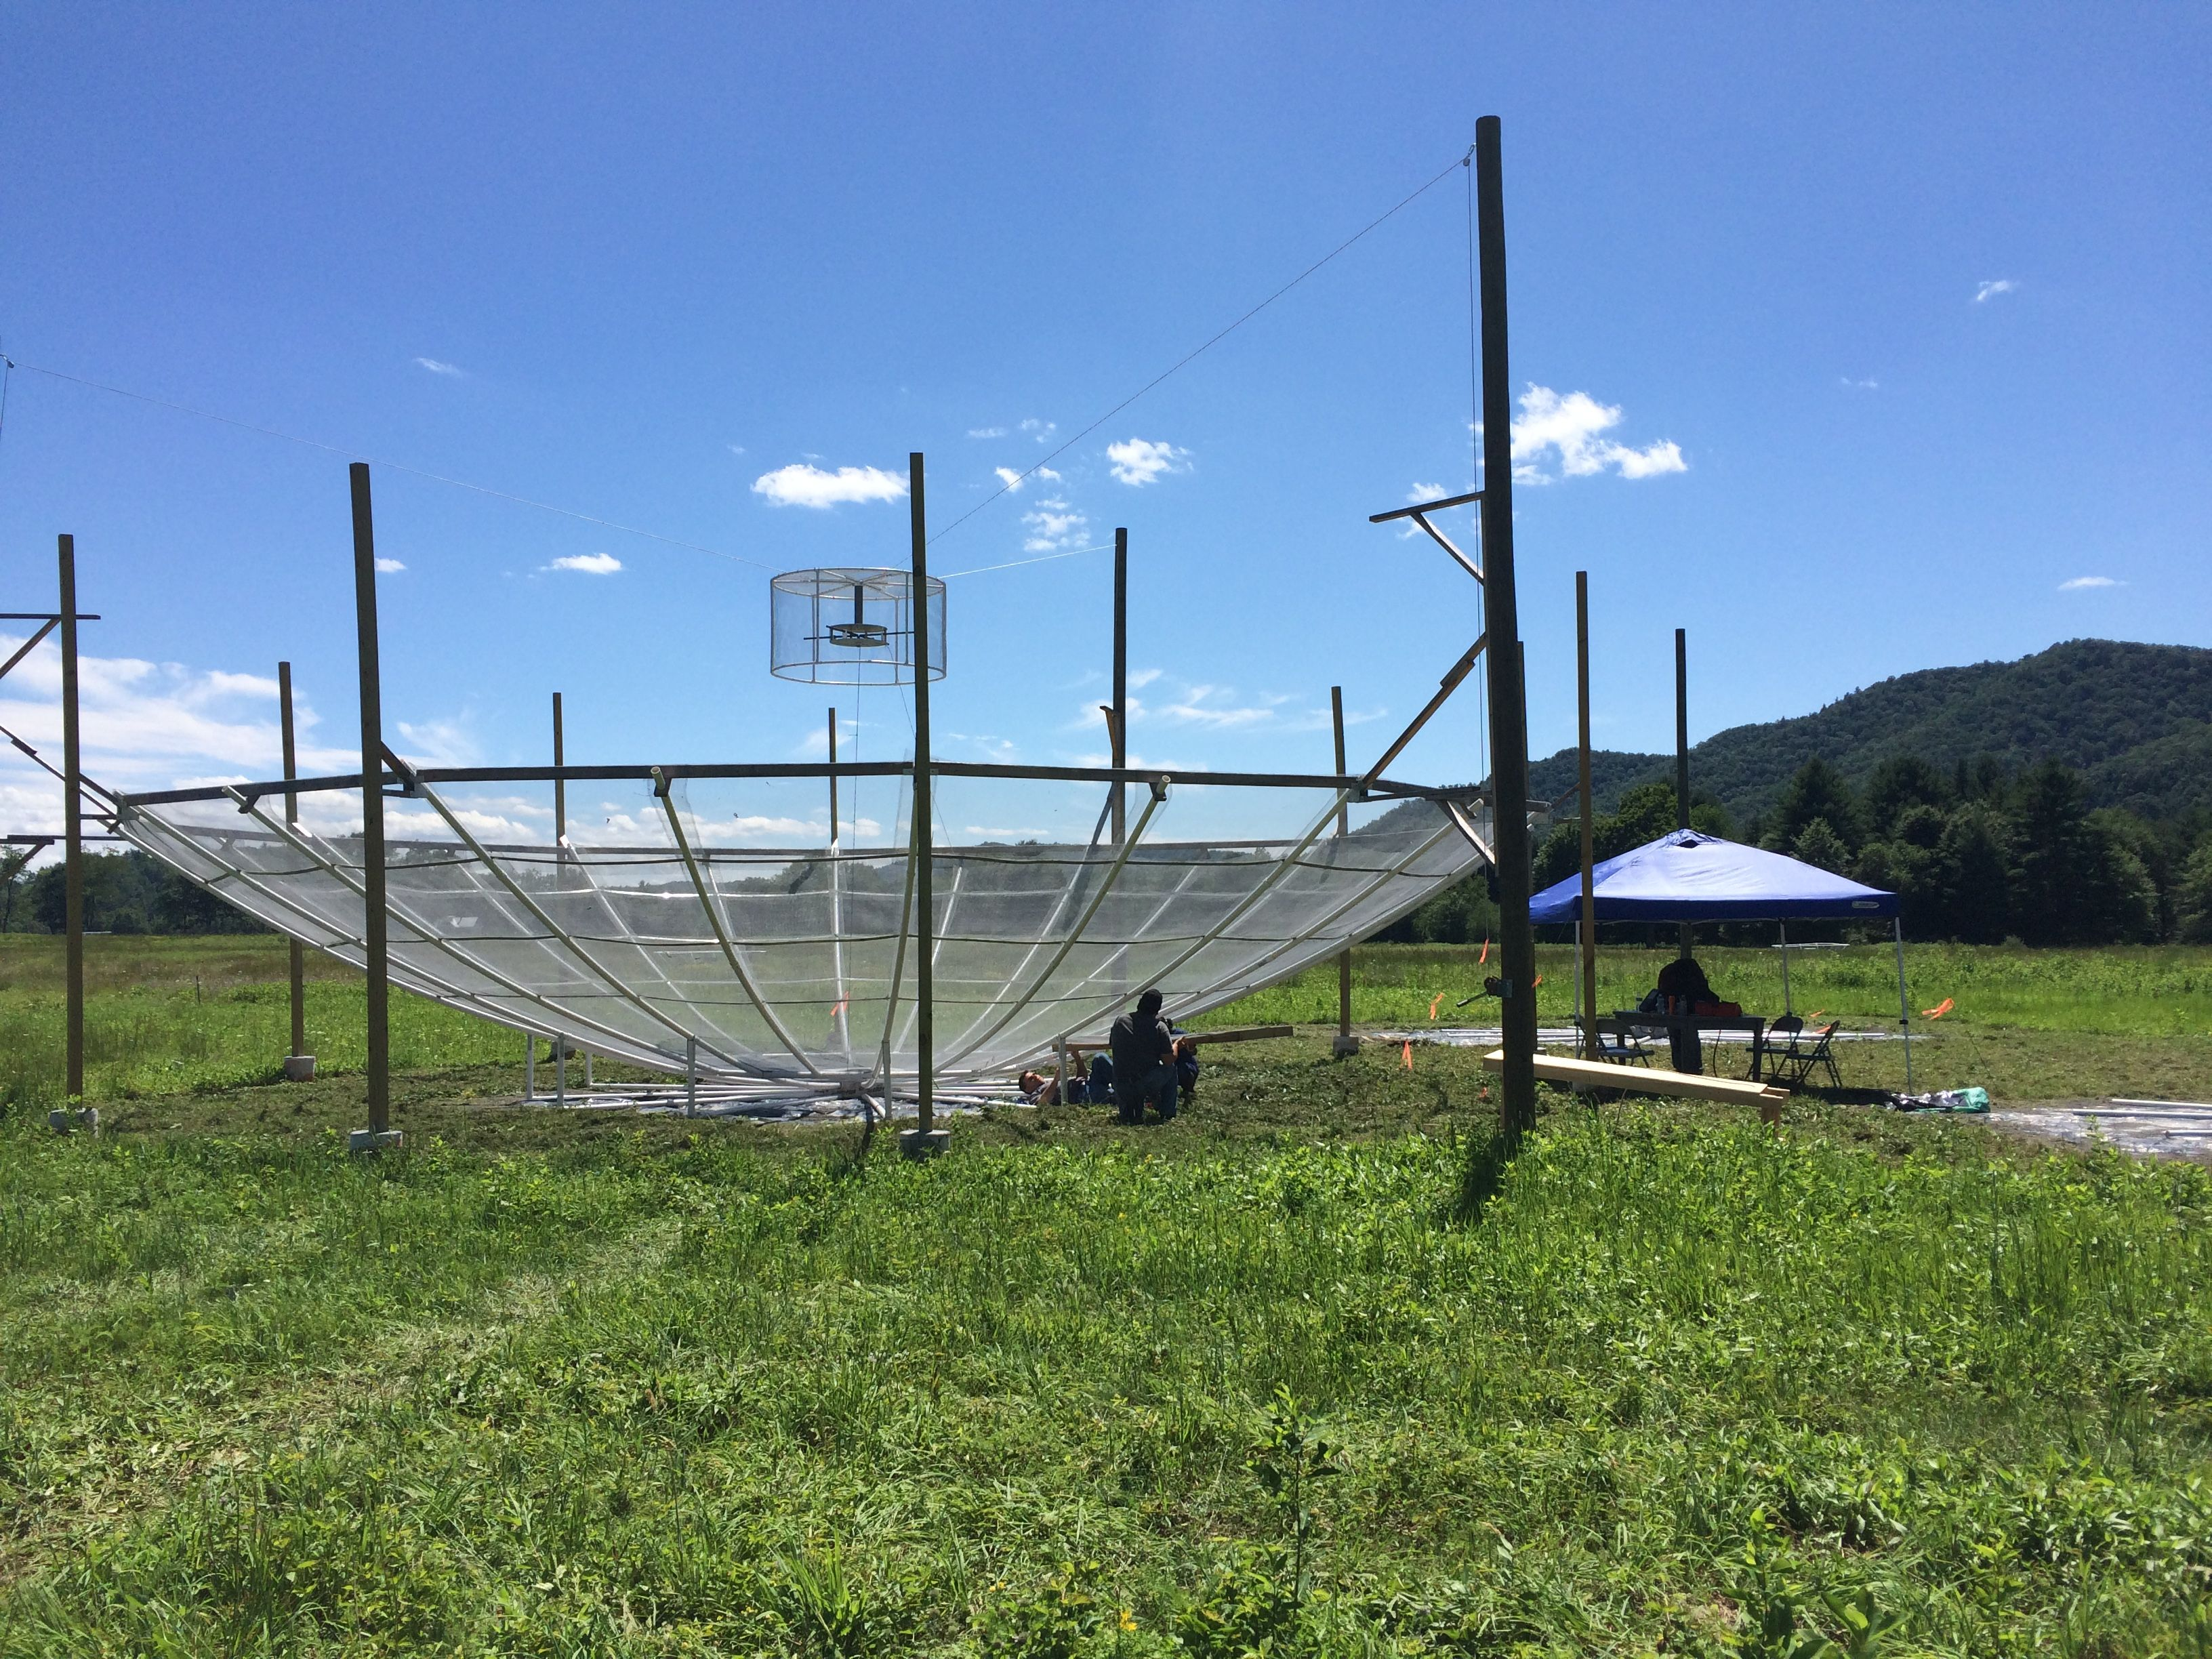
\includegraphics[trim={2cm 20cm 30cm 15cm},clip, totalheight=0.3\textheight]{plots/heradish.jpg}
\caption{HERA dish feed at the Green Bank NRAO site.}
\label{fig:heradish}
\end{figure*}


\section{\textbf{Visibility measurements by a two element interferometer and the delay spectrum}}
Consider a two element interferometer with a baseline $\vec b$. If we denote the electric field sky signal in the direction $\thhat$ by $\volt_\sky(\vec \theta, \nu)$, then the voltage output of each antenna may be written as,  

\begin{equation}
\volt_{1}(\thhat, \nu) = \bmvolt_{1}(\thhat,\nu)\volt_\sky(\thhat,\nu)\nonumber\\
\end{equation}
\begin{equation}
\volt_{2} (\thhat, \nu)= \bmvolt_{2}(\thhat,\nu)\volt_\sky(\thhat,\nu)\fngexp\nonumber\\
\end{equation}
Hence, the time averaged visibility measured by the interferometer may be written as, 
\begin{equation}
\vis(\vec b, \nu) =  \int  \volt_{1}(\thhat,\nu)  \volt_{2}^{*} (\thhat, \nu) \ifngexp d\Omega 
\label{eq1}
\end{equation}

We define the antenna cross power pattern as  $\beam(\thhat,\nu)=\bmvolt_{1}(\thhat,\nu)\bmvolt_{2}^{*}(\thhat,\nu)$ and denote the sky intensity as  $I_\sky(\thhat,\nu)=\volt_\sky(\thhat,\nu)\volt_\sky^{*}(\thhat,\nu)$. Hence, 
\begin{equation}
\vis(\vec b,\nu) = \int \beam(\thhat, \nu) I_\sky(\thhat,\nu) \ifngexp d\Omega
	%	& = & \int B(l,m, \nu) I_{sky}(l,m,\nu) exp(-2\pi i \nu \tau_{g} ) dl dm \nonumber\\
 	%	& = & B(\vec u,\nu) \ast P_{sky}(\vec u,\nu ) \nonumber\\
	%	& = & B(\nu { |\vec b| \over c} , \nu) \ast P_{sky}(\nu { |\vec b| \over c} , \nu) \nonumber\\
	%	& = & B(\tau_{g}, \nu) \ast P_{sky}(\tau_{g} , \nu)	
\label{eq2}
\end{equation}

%i.e, the complex visibility is the Fourier transform of the product of the antenna beam pattern with the sky angular power spectrum. In other words, it is the convolution of the Fourier transform of the antenna power pattern with the Fourier transform of the sky. The complex visibility measured by an interferometer with a given baseline length has explicit dependence on frequency as well as implicit frequency dependence through the spatial frequency $\vec u = \nu { \vec b \over c}$ component. Since $\vec u $ is the For a given baseline length $|\vec b|$, the visibility measured at various frequencies are not only the function of frequencies but also samples different $\vec u$ in the uv space. Delay transformation technique takes the visibility measurements at different frequencies and Fourier transforms the complex visibilities. If we defineI_{sky} the Fourier conjugate of the frequency axis as $\tau$ then the equation could be written as, 
In ~\citet{parsons_et_al2012a}, the Fourier transform of the visibility along the frequency axis was introduced,
resulting in the delay spectrum:
\begin{eqnarray}
\tilde V(\vec b, \tau) & = & \int\!\![{\beam(\vec b,\nu)*I_\sky(\vec b,\nu)] ~e^{-2\pi i\nu\tau}d\nu}%\nonumber\\	                        %& = &   \left [ A(\vec b, \tau)\ast I_{sky}(\vec b, \tau) \ast \delta( \tau - \frac{{\vec {b} \cdot \thhat}}{c} )\right ] d\Omega 
\label{eq3}
\end{eqnarray}
% XXX rethink how to express this equation (not correct about integrated over all sky)
% XXX define tau_g
The convolution is carried out along the $\tau$ axis which is Fourier conjugate of the frequency $\nu$. 
The redshifted 21 cm spatial power spectrum is defined as
\begin{equation}
  P_{21}(k_\perp,k_\parallel) = (|\tilde V(\vec b, \tau)|^{2} \left(\frac{1}{\Omega\Delta B}\right)\left(\frac{D^2\Delta D}{\Delta B}\right)\left(\frac{\lambda^2}{2k_\textrm{B}}\right)^2 ,
\label{eq4}
\end{equation}
where
\begin{equation}
  k_\perp = \frac{2\pi f}{D}\Bigg({b\over c}\Bigg), \text{ }
  k_\parallel = \frac{2\pi\tau\,f_{21}H_0\,E(z)}{c(1+z)^2}, 
 \label{eq5}
\end{equation}
The power spectrum is a function of cosmological as well as instrumental parameters which are:\\
$f_{21}$:rest frame frequency of the 21~cm radiation.\\
$f$: observation frequency.\\
$z$: cosmological redshift corresponding to the frequency of observation.\\
 $\Delta B$: bandwidth centered at the observation frequency.\\
 $k_\textrm{B}$: Boltzmann constant.\\
 $D\equiv D(z)$ comoving distance along the line of sight\\
 $\Delta D$ the comoving distance along the line of sight corresponding to bandwidth of observation $\Delta B$.\\
$E(z)= [\Omega_\textrm{M}(1+z)^3+\Omega_\textrm{k}(1+z)^2+\Omega_\Lambda]^{1/2}$ \\
\indent In this paper, we use $\Omega_{M}=0.27$, $\Omega_{\Lambda}=0.73$, $\Omega_{K}=1-\Omega_{M}-\Omega_{\Lambda}$, $H_0=100 h^{-1}\,$km$\,$s$^{-1}\,$Mpc$^{-1}$, and $P(k_\perp,k_\parallel)$ is in units of K$^2 (h^{-1}$~Mpc$)^3$.

\indent Since both $k_{\perp}$ and $k_{\parallel}$ are functions of the delay $\tau$, corresponding to the given baseline length, the redshifted 21 cm power spectrum could be estimated from the delay spectrum of the visibility measured by an interferometer. The sky delay spectrum from any direction $\thhat$ is convolved with the delay spectrum of the instrument and would be located at the delay $\tau = {\vec b \cdot \thhat \over c}$ %defined this differently earlier
 in the delay domain. The maximum geometric delay possible for a given baseline would be $\tau_{g} ={ b \over c }$ for the direction of $\thhat = 0$, when the phase centre is halfway in between the two antennas. %The phase center is elsewhere defined as being at the center of one of the antennas.
 Hence, the sky contribution from any direction would be confined within $-\tau_{g}<\tau<\tau_{g}$. Due to the chromaticity of the sky signal as well as the instrument response, the delay spectrum of the sky spills over into delays with $\tau> \tau_{g}$, with a decaying amplitude [Ref to the Figure Parsons12]. The foreground, $P_{fg}(\tau)$, which is spectrally smooth, and the 21~cm power spectrum, $P_{21}(\tau)$, which contains spectral signatures, contribute to the sky delay spectrum $P_{sky}(\tau)$.Therefore, in the spill over region $(\tau>\tau_{g})$, the relative strength of the smooth spectrum foreground, with respect to the delay spectrum of the $I_{21}$, reduces and the 21cm delay spectrum could be detectable.

 %In words, the sky delay spectrum from any direction $\thhat$ is convolved with the delay spectrum of the instrument and would be located at the delay $\tau = {\vec b \cdot \thhat \over c}$ in the delay domain. The maximum geometric delay possible for a given base line would be $\tau_{g} ={ b \over c }$ for the direction of $\thhat = 0$ when the phase centre is halfway in between the two antennas. Hence, the sky contribution from any direction would be confined within $-\tau_{g}<\tau<\tau_{g}$. Due to chromaticity of the sky signal as well as instrument reponse, the delay spectrum of the sky spills over the delay $\tau> \tau_{g}$ with decaying amplitude [Ref to the Figure Parsons12]. Sky delay spectrum $I_{sky}(\tau)$ is contributed by the foreground  $I_{fg}(\tau)$  which is spectrally smooth and the 21~cm power spectrum $I_{21}(\tau)$ which contains spectral signatures. Therefore, in the spill over region $(\tau>\tau_{g})$, the relative strength of the smooth spectrum foreground with respect to the delay spectrum of the $I_{21}$ reduces and the 21~cm delay spectrum could potentially be detectable. 


%\subsection{Delay spectrum: An estimate of the 21cm power spectrum}
%Add text here. 
 %\textbf{[ Reference to Nithya's foreground simulation work, reference to any plots on the relative contribution of the  foreground and EoR signal. ]}

\section{\textbf{Effects of multiple reflections on visibility and delay spectrum}}
The Hydrogen Epoch of Reionization Array consists of parabolic dishes which provide increased collecting area per array element compared to its predecessor experiment PAPER. Plane waves incident on a parabolic dish are focussed at the feed which is kept at the focal plane of the dish.
The mismatch between the impedance of free space and the feed and transmission line results in a partial coupling of the sky signal into the feed while the rest is reflected off the feed. 
The reflected signal illuminates the dish and most of it is reflected back into the space.
However, a part of it reflects back and forth several times in between the feed and the vertex of the dish which is shadowed by the feed.
Such reflections generate multiple copies of the incident sky signal of reduced strength at various delay and phase and thus produces spurious correlations in the visibilities of interferometric data.  Identical spurious visibilities could be resulted due to reflections internal to the system causing delay space distortion. Therefore, it is necessary to measure and understand the instrument delay spectrum in order to qualify the system for the measurement of 21cm power spectrum. 
In this section we compute the visibility of a two element interferometer accounting for the additional reflections of the sky signal in between the feed and the dish vertex and the corresponding effects on the delay spectrum in detail. We assume two antennas with identical geometry and electrical parameters i.e, $\bmvolt_{1}(\thhat,\nu)=\bmvolt_{2}(\thhat,\nu) = \bmvolt(\thhat,\nu)$. 
 \subsection{\textbf{Antenna Reception With Multiple Reflections}}
\label{sec:multiple}
To examine the performance of an antenna and feed in the presence of multiple reflections, we can think of the system as a screen at a distance $F$ from a feed (see Figure \ref{fig:sys}), noting that this does ignore the sky pattern of the feed itself.  The screen reflects a factor, $\Gamma_d$, of the voltage and transmits $(1+\Gamma_d)$ (see, {\em e.g.} Pozar).  Similarly, the feed reflects $\Gamma_f$ and transmits $(1+\Gamma_f)$.  The voltage pattern $\volt_{sky}$ is incident onto that system and  $(1+\Gamma_{d})(1+\Gamma_{f})$ is coupled into the cable leading from the feed. 
Additionally, however, the voltage pattern is reflected off the feed ($\Gamma_f$), then the dish ($\Gamma_d$) and subsequently $(1+\Gamma_{f})$ of it reenters the feed with a roundtrip time delay $\Delta \tau=2F/c$. Hence, if $v_{sky}$ is reflected $n$ times in between the feed and the dish, the net voltage entering the feed after the
$n^{th}$ reflection may be written as:
\begin{eqnarray}
\volt_{rec} & = &  (1+\Gamma_d) (1+\Gamma_{f}) \volt_{sky}[1+ \Gamma_{f}\Gamma_{d} \dfngexp \nonumber \\
	&& + (\Gamma_{f}\Gamma_{d})^2  (\dfngexp)^{2}+ \nonumber \\
&&  ....+ (\Gamma_{f}\Gamma_{d})^{n} (\dfngexp)^{n}]
\label{eq6}
\end{eqnarray}


\begin{figure}
\centering
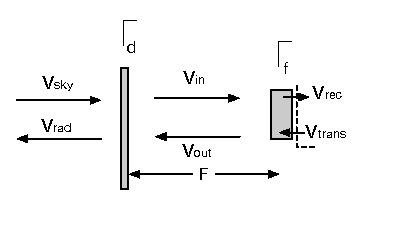
\includegraphics[width=0.5\textwidth]{plots/microsys.pdf}
\caption{System}
\label{fig:sys}
\end{figure}

\noindent
%Defining $a=\volt_{rec}/\volt_{sky}$ and we see that 
Hence,
 \begin{eqnarray}
{\volt_{rec}\over \volt_{sky} } & = &   (1+\Gamma_d)(1+\Gamma_{f}) \displaystyle\sum\limits_{n=0}^{N} [\Gamma_{f}\Gamma_{d}\dfngexp]^{n}\nonumber\\
& = & \frac{ (1+\Gamma_d)(1+\Gamma_{f})}{1+\Gamma_{f}\Gamma_{d}\dfngexp} 
\label{eq7}
\end{eqnarray}
Note that $n=0$ is when the initial wave enters the cable at the feed (where we assume we have set our reference plane).  We may identify $(1+\Gamma_d)$ as the voltage reception pattern of the antenna, denoted $\bmvolt(\thhat,\nu)$, which is a function of angle on the sky.  Additionally, $(1+\Gamma_f$) is the voltage efficiency for the feed (not a function of angle).

%As an aside, note that the sum in Eq. \ref{eq:Sigma} may be evaluated we may rewrite
%\begin{equation}
%{\volt_{rec}\over \volt_{sky} } =  (1+\Gamma_d)(1+\Gamma_{f})\frac{1+\Gamma_{f}^{N+1}\Gamma_{d}^{N+1}(\dfngexp)^{N+1}}{1+\Gamma_{f}%\Gamma_{d}\dfngexp} \nonumber
%\end{equation}
%which, in the limit becomes:
%\begin{equation}
%{\volt_{rec}\over \volt_{sky} } = \frac{ (1+\Gamma_d)(1+\Gamma_{f})}{1+\Gamma_{f}\Gamma_{d}\dfngexp} \nonumber
%\end{equation} 
%since $|\Gamma_d|$ and $|\Gamma_f|$ are less than one.

An accurate measurement of this quantity requires receiving $v_{sky}$ from a well calibrated, wideband source in the sky in the far field of the HERA antenna element with significant isotropic emission. While this condition is hard to achieve in practice, due to the reciprocity of the antenna performance in the transmission and reception mode, the right hand side of equation \ref{eq:Sigma} could be measured using the return loss measurement technique with a vector network analyzer (VNA). \\

\section{\textbf{Reflectometry measurements}} 

Reflectometry measurements are carried out at the HERA element prototype in Green
Bank, WV (Figure \ref{fig:heradish}) in order to measure the instrument response of the feed and dish assembly and characterise the performance.  HERA element consists off a $14\,m$ diameter
parabolic reflector and a crossed-dipole pair as a feed. The cross dipole antenna pair is identical to the feed of the PAPER antenna which is suspended at the focal plane of the dish with the support of three vertical poles. HERA elements are closely spaced with centre to centre distance between two dishes are equal to the dish diameter. Therefore, to reduce the coupling between the adjacent dishes, the crossed dipole feed along with the back plane is encased in a cylindrical cage. The feed is raised and
lowered by a three-pulley system mounted on the three poles. The focal height of the dish is $5m$.  The detail geometry and electromagnetic design of of the feed is presented in deBoer et al 2016. \\
%A vector network analyser is connected via a 50feet long cable at the feed output of the HERA element and the return loss $(s_{11})$ of the HERA element is measured as a function of frequencies while the feed is suspended at the focal plane of the dish. 

 A VNA is connected to the HERA element via a 50-foot cable. It then transmits a broadband noise voltage, $\volt_{trans}$, and a factor $(1+\Gamma_f)$ of this voltage is radiated by the feed while the fraction $\Gamma_{f}$ returns to the VNA. Although the radiated signal illuminates the dish and most of it is radiated into free space, a fraction $\Gamma_d$ of this signal is reflected back towards the feed, and $(1+\Gamma_f)$ is received by the VNA.  The received voltage, after $n$ reflections between the dish and the feed (where again $n=0$ is the first reflected signal at the reference plane), is therefore:

\begin{eqnarray}
\volt_{rec} & = &  \Gamma_f \volt_{trans} \nonumber \\
         && + \volt_{trans} (1+\Gamma_f)^2 \Gamma_{d} \dfngexp \nonumber \\
         && + \volt_{trans} (1+\Gamma_f)^2 \Gamma_{d} \dfngexp \Gamma_d\Gamma_f\dfngexp \nonumber \\
         && + \volt_{trans} (1+\Gamma_f)^2 \Gamma_{d} \dfngexp (\Gamma_d\Gamma_f\dfngexp)^2 \nonumber \\
&&  ....+ \volt_{trans} (1+\Gamma_f)^2 \Gamma_{d} \dfngexp (\Gamma_d\Gamma_f\dfngexp)^n \nonumber \\
\label{eq8}
\end{eqnarray}
Therefore, 
\begin{equation}
{\volt_{rec}\over \volt_{trans} } = \Gamma_f + \frac{(1+\Gamma_f)^2}{\Gamma_{f}} \displaystyle\sum\limits_{n=1}^{N} [\Gamma_{f}\Gamma_{d}\dfngexp]^{n}
\label{eq9}
\end{equation}
The VNA measures the quantity $\volt_{rec}/\volt_{trans}=s_{11}$ which is the voltage reflection coefficient of the HERA element.
The fundamental differences between the right hand side of equations \ref{eq:Sigma} and \ref{eq:s11} are the $n=0$ term and the multiplicative factor in front of the convergent series $\displaystyle\sum\limits_{n=1}^{N} [\Gamma_{f}\Gamma_{d}\dfngexp]^{n}$ that represents the contribution of the delayed voltage components at the VNA input, arising due to multiple signal reflections between the feed and the dish. Finally, writing $\volt_{rec}/\volt_{trans}=s_{11}$, equation \ref{eq:s11} can be written as,
\begin{equation}
s_{11} +\frac{(1+\Gamma_f)^2}{\Gamma_f}-\Gamma_f = \frac{(1+\Gamma_f)^2}{\Gamma_{f}} \displaystyle\sum\limits_{n=0}^{N} [\Gamma_{f}\Gamma_{d}\dfngexp]^{n}
\label{eq10}
\end{equation}
Comparing to Eq. \ref{eq:Sigma} and we find that
\begin{eqnarray}
{\volt_{rec}\over \volt_{sky} } & = & (1+\Gamma_d)\left[(1+\Gamma_f) + \frac{\Gamma_f}{(1+\Gamma_f)}\left(s_{11} - \Gamma_f\right)\right] \nonumber\\
 & = & \bmvolt(\thhat,\nu) \left[(1+\Gamma_f) + \frac{\Gamma_f}{(1+\Gamma_f)}\left(s_{11} - \Gamma_f\right)\right]
\label{eq11}
\end{eqnarray}
When the feed return loss is measured separately, all the higher order terms of equation \ref{eq:s11} do not exist. In this case, $\Gamma_f = s_{11}^{f}$. Using this measurement and the VNA measurement of $s11$, the quantity $v_{rec}\over v_{sky}$ is estimated. \\
%
\indent From this, for a two element interferometer with identical antenna elements, the ratio of the received sky intensity to true sky intensity will be, 
\begin{eqnarray}
{I_{rec}\over I_{sky} } & = & \Bigg|{\volt_{rec}\over \volt_{sky} }\Bigg|^2 =  \beam(\thhat,\nu)\times \nonumber\\
             && \left[|1+\Gamma_f|^2 +  2\operatorname{Re}\left(\frac{\Gamma_f}{(1+\Gamma_f)}(s_{11} - \Gamma_f)\right)\right] + \nonumber\\ 
             &&  \left[ \frac{|\Gamma_f|^2}{|1+\Gamma_{f}|^2}|s_{11} - \Gamma_f|^2  \right]  \nonumber\\
\label{eq12}             
\end{eqnarray}

In terms of visibility, the same could be written as,  
\begin{eqnarray}
\vis^{mul}(\vec b,\nu) & = & \int \beam(\thhat,\nu)\times \nonumber\\
             && \left[|1+\Gamma_f|^2 +  2\operatorname{Re}\left(\frac{\Gamma_f}{(1+\Gamma_f)}(s_{11} - \Gamma_f)\right)\right] + \nonumber\\ 
             &&  \left[ \frac{|\Gamma_f|^2}{|1+\Gamma_{f}|^2}|s_{11} - \Gamma_f|^2  \right]  I_{sky} \ifngexp d\Omega
\label{eq13}
\end{eqnarray}

Comparing equations \ref{eq:power_ratio} and \ref{eq2}, the cross power generated by $v_{1}$ and $v_{2}$ would have a spurious visibility response due to the mutual correlation between multiply reflected voltages represented by the second and the third term of the right hand side of equation \ref{eq:power_ratio}. In the ideal case, $\Gamma_{f}=0$, in which case equation \ref{eq:power_ratio} results in equation \ref{eq2}. The Fourier transform of this visibility spectrum along the frequency axis results in the delay spectrum. 
In the delay domain, visibilities contributed to by any two voltage components from two antennas with no mutual delay will be located at the delay $\tau = 0$ whereas any two voltage components from two antennas having a mutual delay of $n\Delta \tau$ will be centred at $n\Delta \tau$. These will broaden the width of the delay spectrum, which ultimately interferes with the 21cm power spectrum detection.

\begin{figure*}
\centering
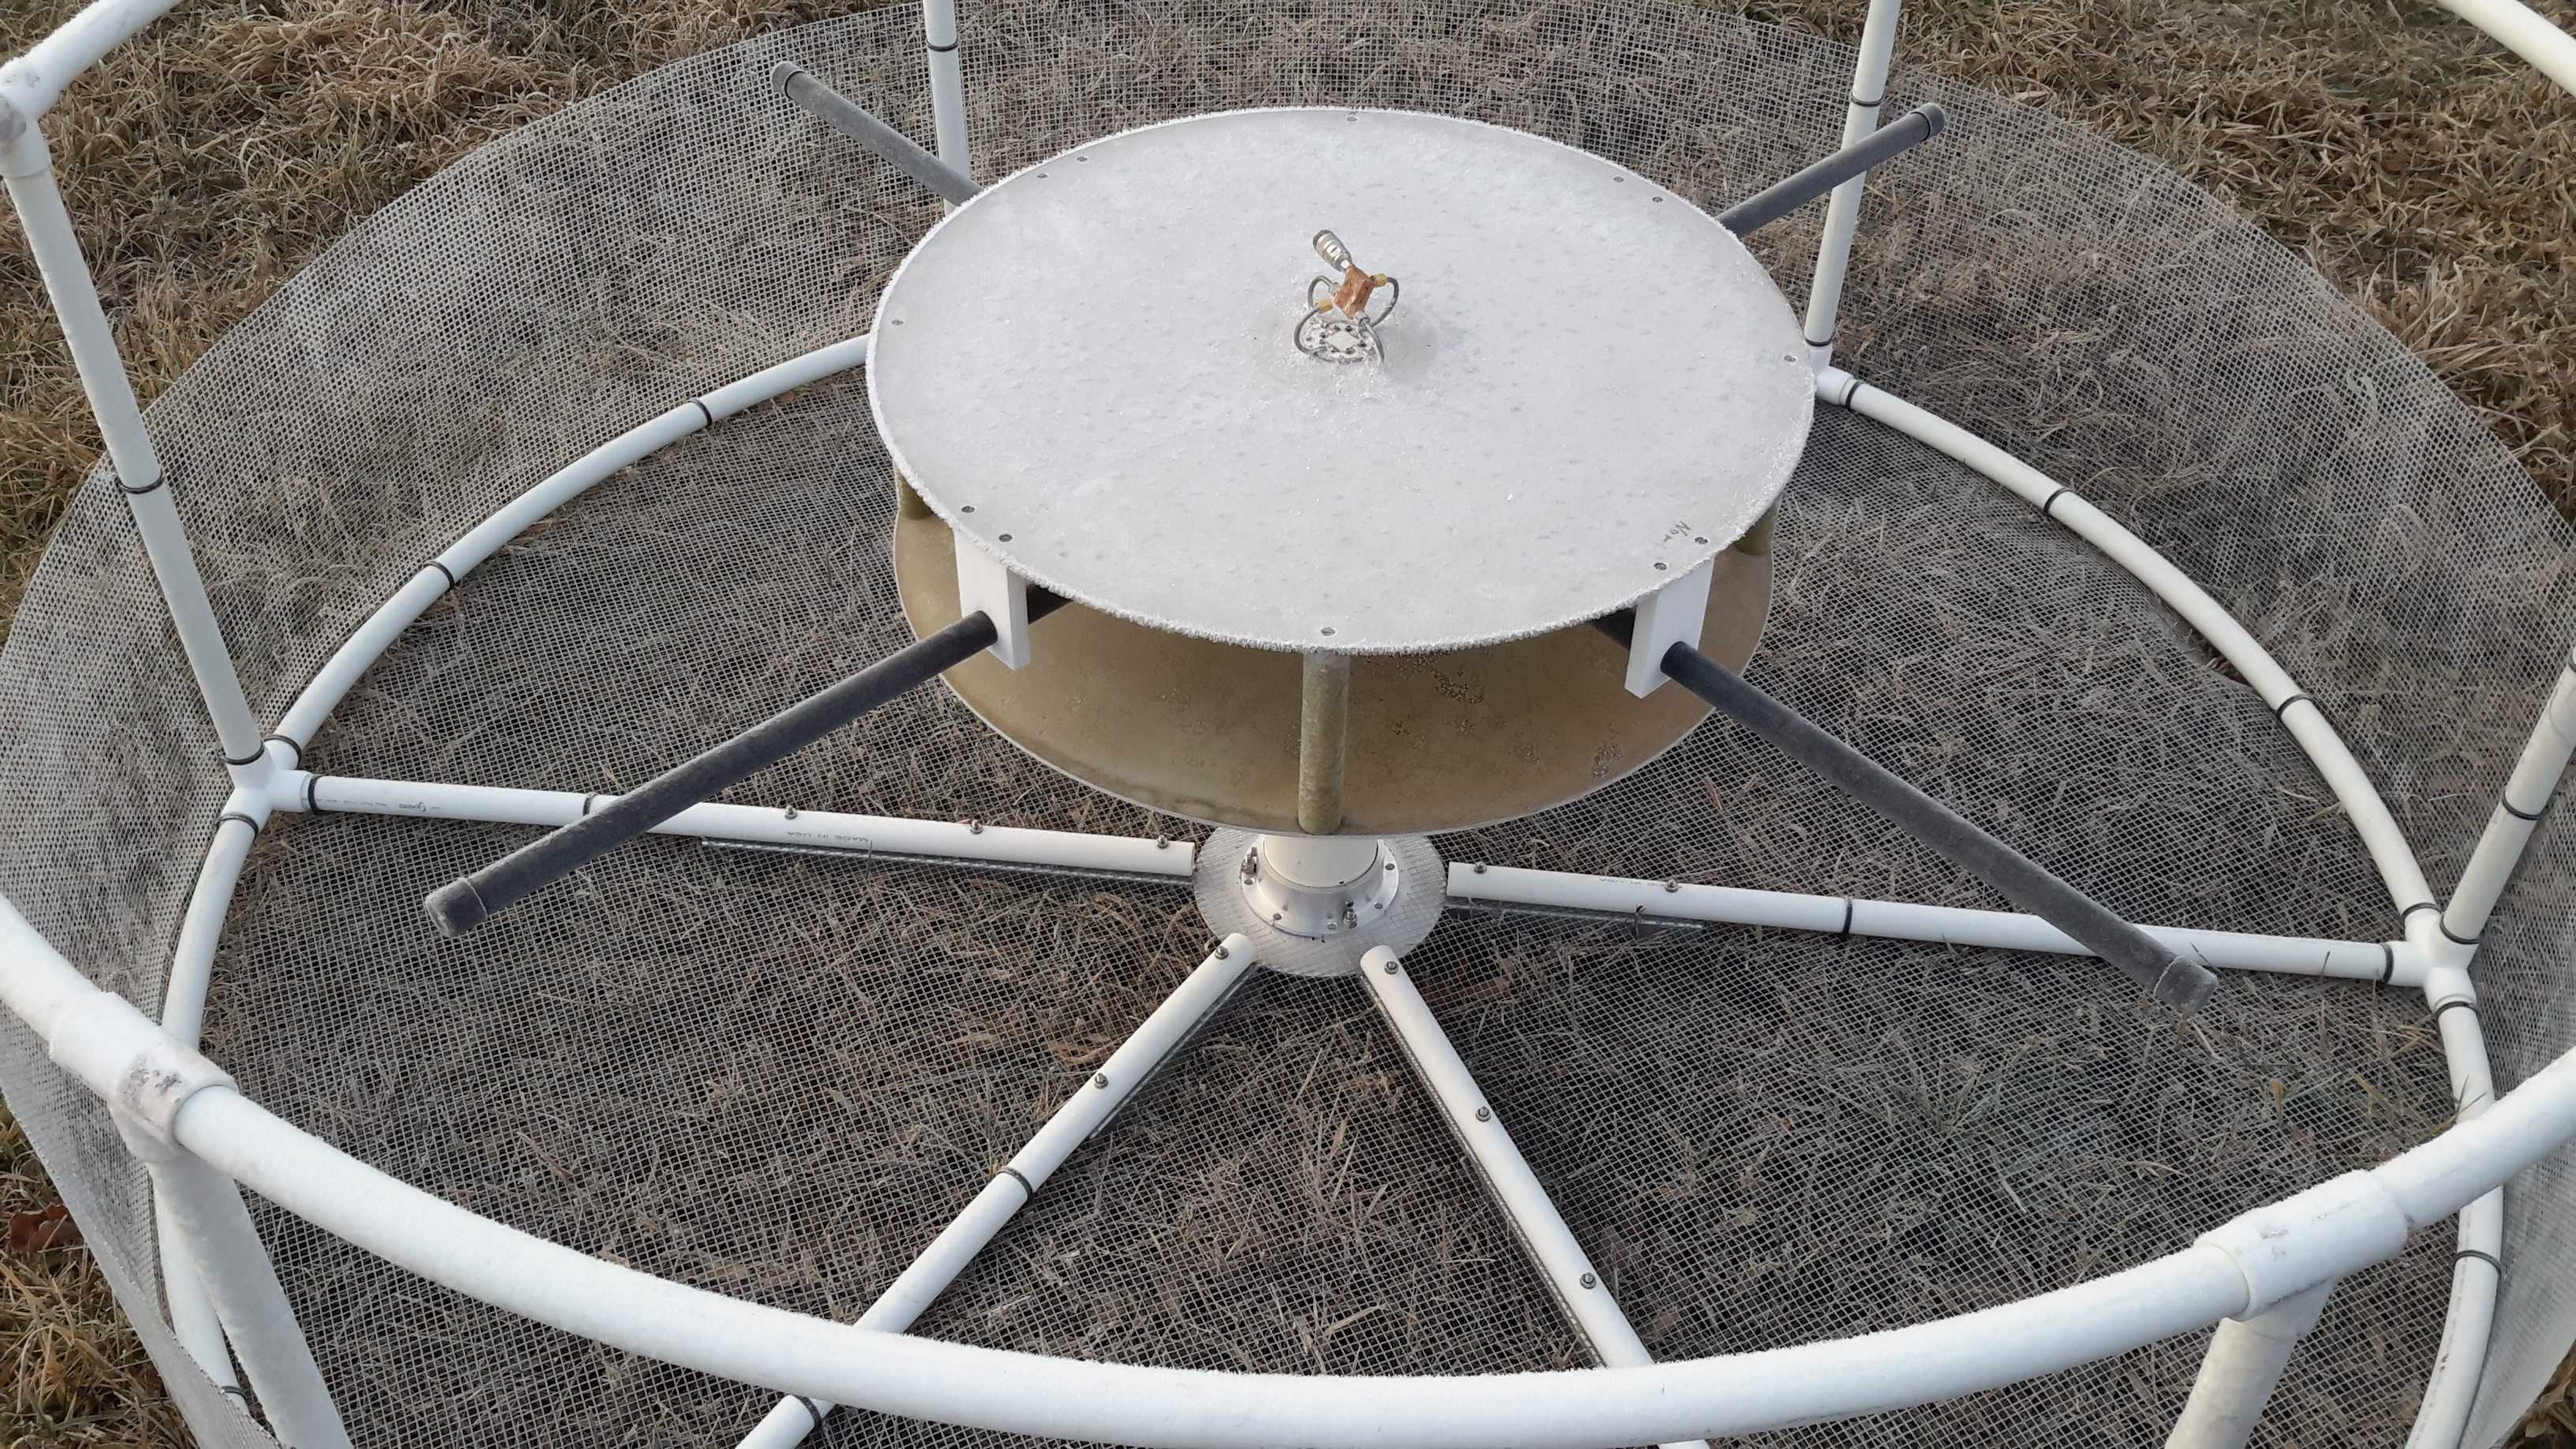
\includegraphics[trim={2cm 10cm 20cm 5cm},clip, totalheight=0.3\textheight]{plots/herafeed.jpg}
\vspace{1.0 em}
\caption{The HERA feed consists of a pair of crossed-dipoles over 1.72 mt diameter backplane made of wire mesh. The backplane is surrounded by 0.36 m wide wire mesh around the edge resulting in encasing the crossed-dipoles in a cylindrical cage.}
\label{fig:herafeed}
\end{figure*}


\section{Results}
Return loss measurements yields the instrument pass band response that would manifest in autocorrelation data of a single HERA element. Upon our assumption that two adjacent antenna elements have identical design parameters and electrical properties, this power is also a measure of the cross power or the visibility $\vis (\vec b, \nu)$ between the two antennas with a normalisation factor of $2$. 

The simultated and measureded return loss of the feed as well as the HERA element is shown in figure \ref{RL_mag_feed} and figure \ref{RL_mag_dish}. The measurements deviates from the simulated performance in one major aspect. While the return loss of the simulated structure shows two resonant peaks around 120 and $160~MHz$, the feed resonance occur at slightly higher frequencies. While the simulated response shows very wide resonant peaks, as expected from these dipole structures, the measured return loss of the feed has a narrow peak around its low frequency resonance. This feature somewhat dominates the fall off rate in the delay response of the system bandpass. The delay response of the feed alone is shown in figure \ref{ds_feed_on_dish_trans} along with the delay response of a HERA element in transmission mode. In the following sections, we compute the response of the HERA element in the receiving mode. 
\begin{figure}[ht]
\begin{minipage}[b]{\linewidth}
\centering
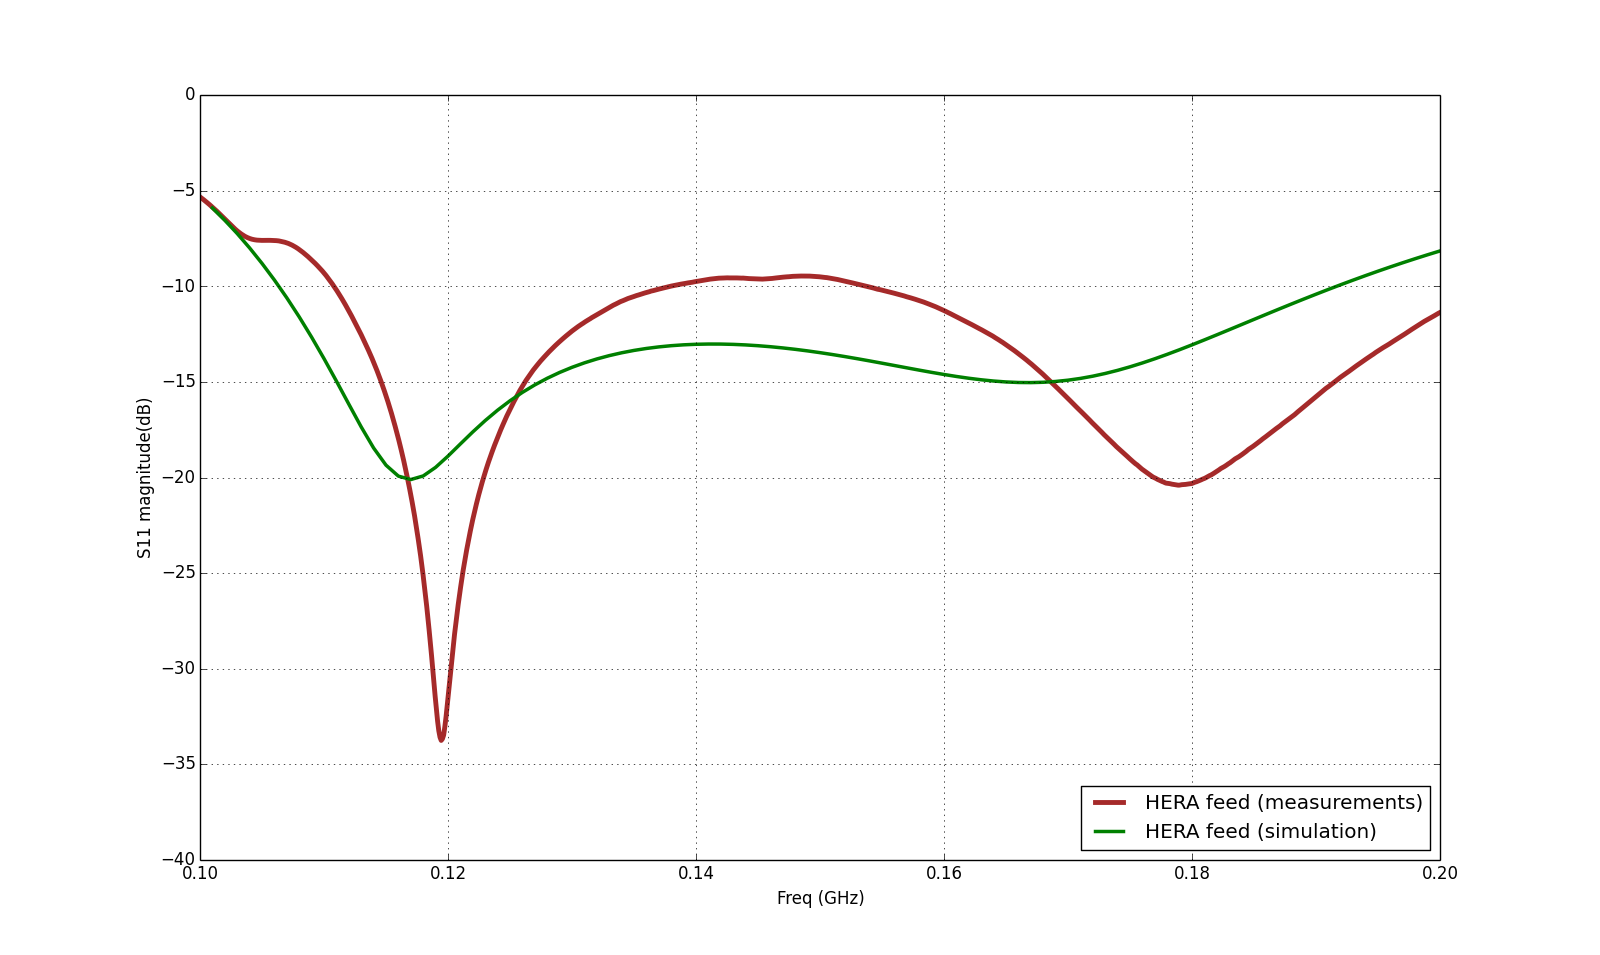
\includegraphics[angle=0, width=\linewidth]{GB_reflectometry_part3/plot/RL_mag_feed.png}
\end{minipage}
\vspace{0.1cm}
\begin{minipage}[b]{\linewidth}
\centering
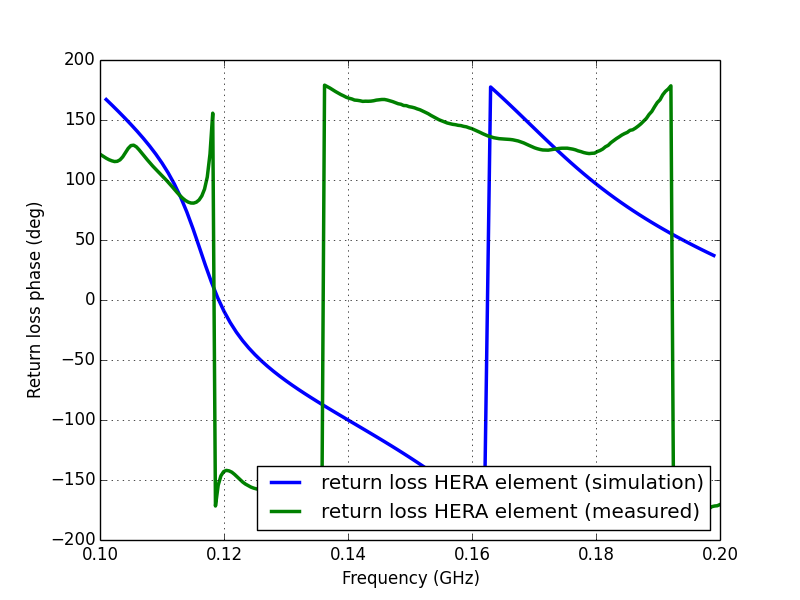
\includegraphics[angle=0, width=\linewidth]{plots/feed_meas_sim_ph.png}
\end{minipage}
\caption{Magnitude and phase of the return loss of the feed as simulated and measured. While both the measurement and the simulation shows similar resonance around $120~MHz$, the simulation shows a better matching to a 50 Ohm transmission line compared to the measurements. The measurement also has some small scale fluctuation due to multiple reflection of the signal at the VNA input. }   
\label{RL_mag_feed}
\end{figure}



\begin{figure}[ht]
\begin{minipage}[b]{\linewidth}
\centering
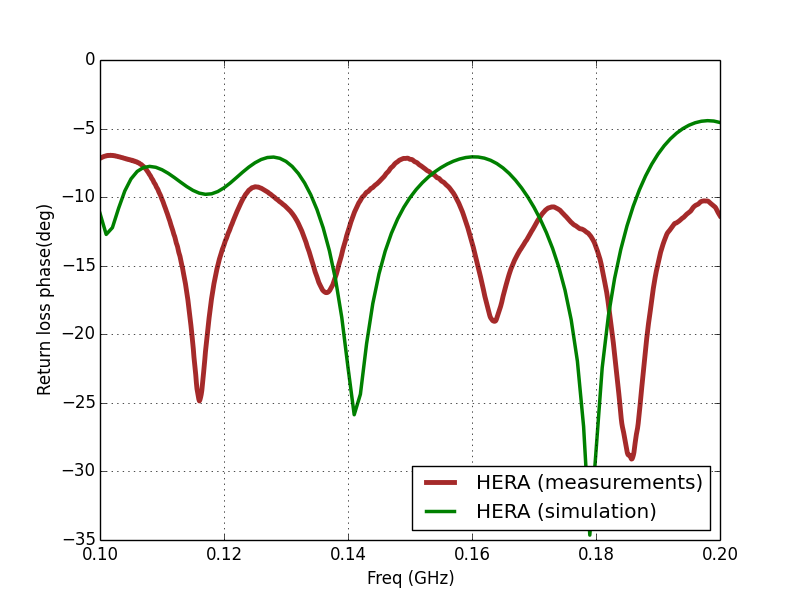
\includegraphics[angle=0, width=\linewidth]{GB_reflectometry_part3/plot/RL_mag_dish.png}
\end{minipage}
\vspace{0.1cm}
\begin{minipage}[b]{\linewidth}
\centering
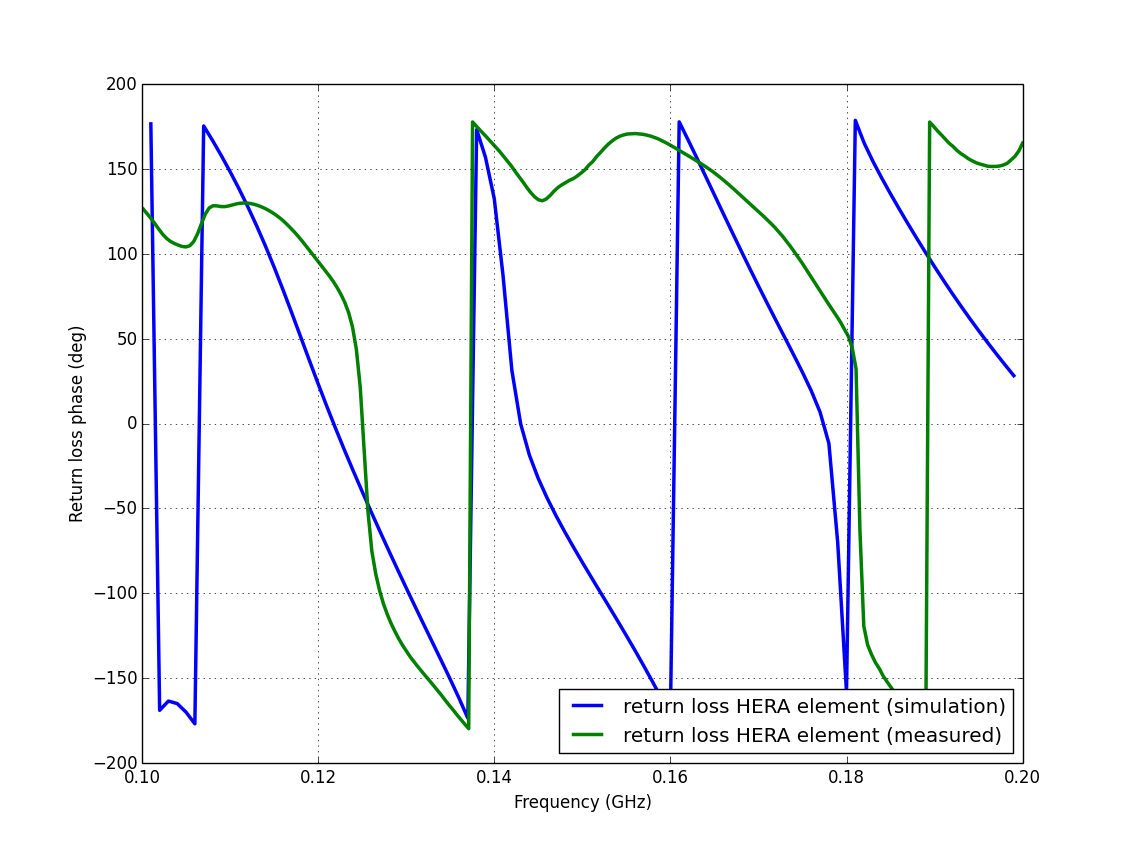
\includegraphics[angle=0, width=\linewidth]{plots/HERA_meas_sim_ph.png}
\end{minipage}
\caption{Magnitude and phase of the return loss of the HERA element as simulated and measured. In this case, both measurement and simulation shows similar level of return loss across the band with marginally better return loss at the high frequency end of the band. }   
\label{RL_mag_dish}
\end{figure}

\begin{figure}       
\centering
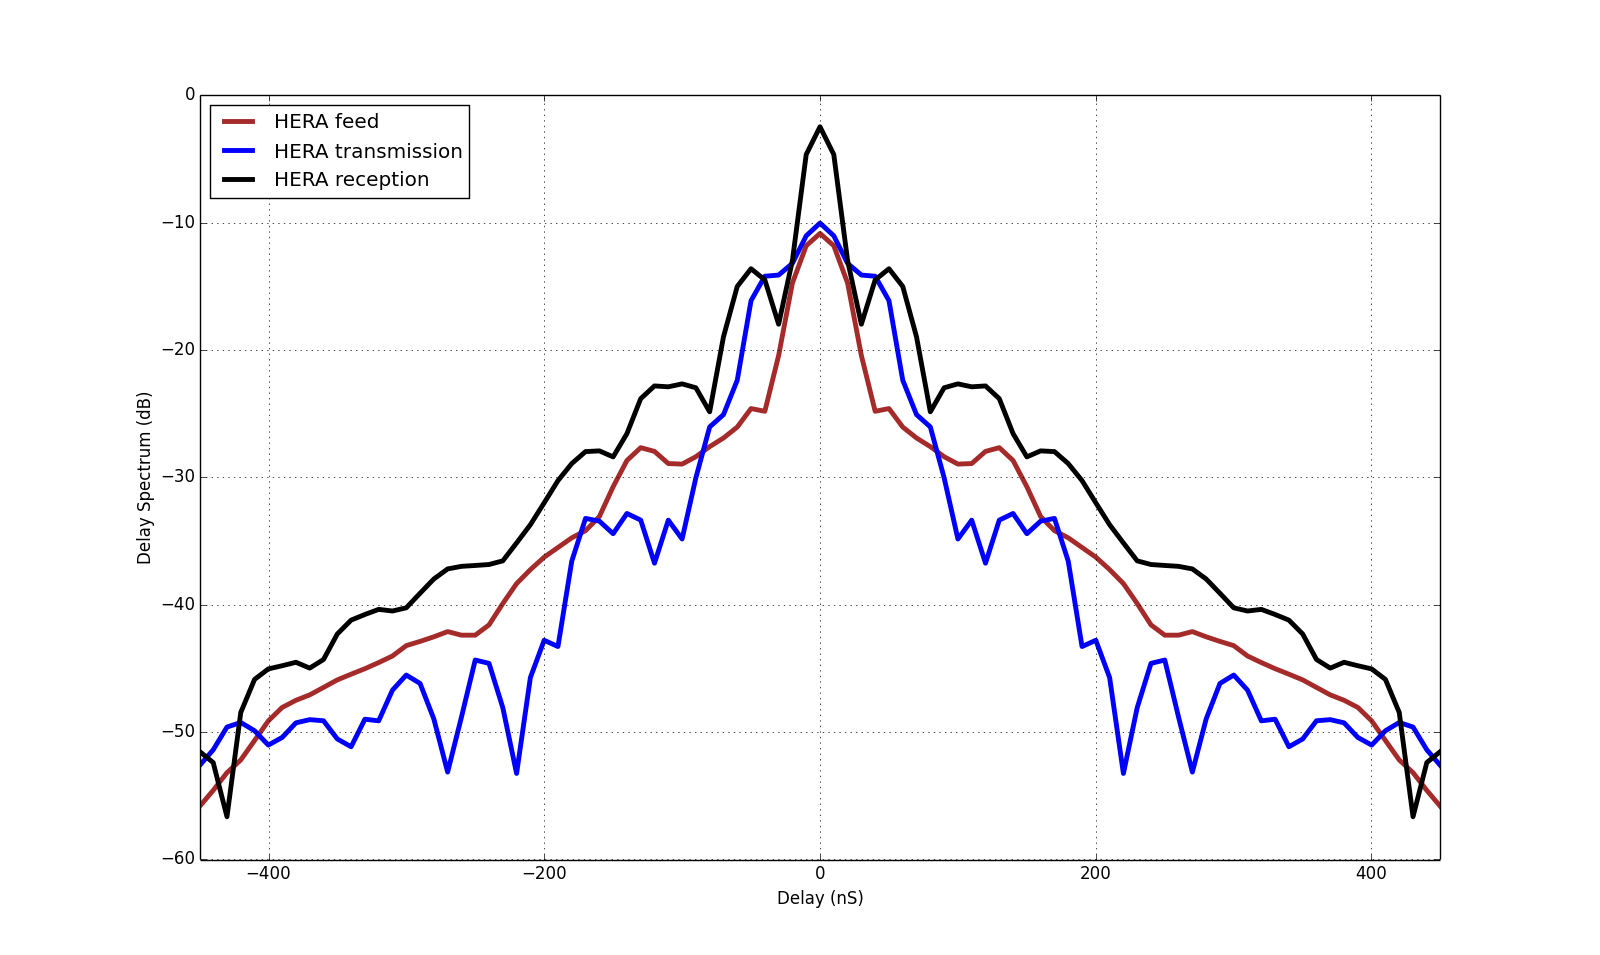
\includegraphics[width=\linewidth]{GB_reflectometry_part3/plot/ds_feed_on_dish_trans_recp.png}
\caption{Delay spectrum of the HERA feed (brown) estimated by taking the Fourier transform of the measured return loss of power at the feed output. The feed, when suspended on the dish results in a more complex return loss as shown in figure \ref{RL_mag_dish} and corresponding delay response is shown here in black. This figure shows the delay spectrum of the instrument in the as estimated from direct measurements of the return loss i.e, in the transmission mode of the antenna. }
\label{ds_feed_on_dish_trans}
\end{figure}

Figure \ref{RL_mag_dish} shows the measured return loss when the feed is suspended at the focal plane of the parabolic dish which is at $5m$ from the dish vertex. The measured return loss is much more complex than what is found from the simulation. The delay spectrum in the transmission mode is shown in \ref{ds_feed_on_dish_trans}. To estimate the delay spectrum of the dish-feed assembly i.e one single HERA element, this measurement is first corrected to map the response of the antenna from transmitting mode to receiving mode via equation \ref{zero_delay_correction}. The corrected measurement is then Fourier transformed to obtain the delay spectrum of the instrument in the receiving mode as given in equation \ref{corrected_response}. Measurement bandwidth is kept much larger than the bandwidth of operation to achieve higher delay resolution. A number of systematic effects as well as mathematical artfacts that are critical to this measurements and their effects on the corresponding estimation of the delay spectrum are taken in to account in determination of the delay spectrum and described below. 

\subsection{\textbf{Zero delay correction}}
%At first, the frequency domain measurement of s11 is Fourier-transformed to compute the response of the system in the delay domain. 

While measuring the return loss of the dish-feed assembly, the signal transmitted by the VNA is reflected first off the feed. This is represented by $\Gamma_{f}$ in equation \ref{eq:power_ratio}. This essentially represents a mismatch in between the feed and the 50 Ohm transmission line. In delay domain, this appears at the zero delay bin. The zero delay response is identical whether or not the feed is suspended on the dish. Therefore, we measure this response by measuring the feed return loss alone while the feed is kept on the ground facing the sky. This results in feed return loss alone including the surrounding cage structure but excluding the dish response. While $\Gamma_{f}$ fraction of incident voltage is reflected off the feed, $1+\Gamma_{f}$ fraction of the voltage is transmitted. In receiving mode, upon initial incidence, $\Gamma_{f}$ fraction of voltage is reflected back in to the space while $1+\Gamma_{f}$ voltage enters the feed. In receiving mode, in delay domain, this appears at the zero delay bin.
The using the return loss measurement of the feed $(\Gamma_{f})$, the return loss measurement $s_{11}$ of the dish and feed assembly is corrected via equation \ref{eq:power_ratio} and the quantity of interest ${I_{rec}\over I_{sky}}$ is estimated. 

%\subsection{\textbf{Antenna beam pattern and feed return loss}}
%The return loss $\Gamma_{f}$ determines the amount of power coupled to the system via the feed antenna. Additionally, with each reflections, the power coupled to the system reduces by a factor of $\Gamma_{f}^{2}$. Since reflected signal results in system response in higher delay, multiple reflections of the signal off the feed and the dish would result in an exponential envelope in the delay spectrum.  The return loss of power results from the antenna impedance mismatch with the free space as well as the transmission line. While antenna beam pattern $A_{f}$ is a smooth function of frequency and should have its imprint confined to lower delays, the return loss $\Gamma_{f}$ broadens the delay spectrum. However, a smaller return loss will result in vertical shift of the delay spectrum at lower values and therefore can make the higher order reflections insignificant. 
During observation, each HERA element is connected to an active balun similar to the ones used in the PAPER antenna (need reference) which provides greater than 10dB return loss of power at the feed output.These baluns are under further design improvements aiming at 10 to 20dB better imepedance match between the feed and the balun than the measurements presented here.  Our measurement is done using a vector network analyser for which the active balun has been replaced by a passive balun.Given the antenna impedance and the 50 Ohm transmission line the measurements are done using the passive balun with a 4:1 impedance ratio providing a net return loss of power between the sky, the antenna and the transmission line shown in the figure \ref{RL_feed_mag}. This measurements are conservative estimate  for both $\Gamma_{f}$ and $s_{11}$.

\subsection{\textbf{Dish reflections}}
Measurement equations shows the effects of multiple reflections of the sky signal between the feed and the dish. Any other reflections off the feed structure and/or any other part of the dish-feed assembly would appear at arbitrary delays. The estimated delay spectrum of the instrument is collectively contributed by all the reflections. Delay spectrum estimated from the return loss measurement of the feed alone,  provides the lowest limit of the delay spectrum of the instrument considering there is no multiple reflections in between the feed and the dish. 
From figure \ref{ds_feed_on_dish_trans}, at lower delays, the reflections are dominated by the feed structure. Therefore, the delay spectrum in both the cases follow each other. Since the distance between the feed and the dish is 5 m, the roundtrip delay between the dish and the feed as about $30~ns$ around which these two delay spectrum starts to deviate. At delays $\> 50nS$ the dish reflections starts to dominate over the reflections from the feed structure and the two delay spectrum deviates from each other. 

\subsection{\textbf{Measurement bandwidth and window function}}
Estimation of the delay spectrum by taking the Fourier transform of the measured return loss is sensitive to the bandwidth of measurements. Since the measurements are done in the spectral domain, measurement between two frequencies is analogous to windowing the frequency domain data by a square window function. In the delay domain, Fourier transform of this would result in multiple side lobes at higher delays. Therefore, appropriate windowing of the data is  necessary prior to taking the Fourier transform of the measured data. Figure \ref{fig:window} shows the delay spectrum estimated from the measured data using a square window as well as Blackman Harris window. Windowing the data prior to Fourier transform significantly reduces the system response higher delays.  
\begin{figure}
\centering
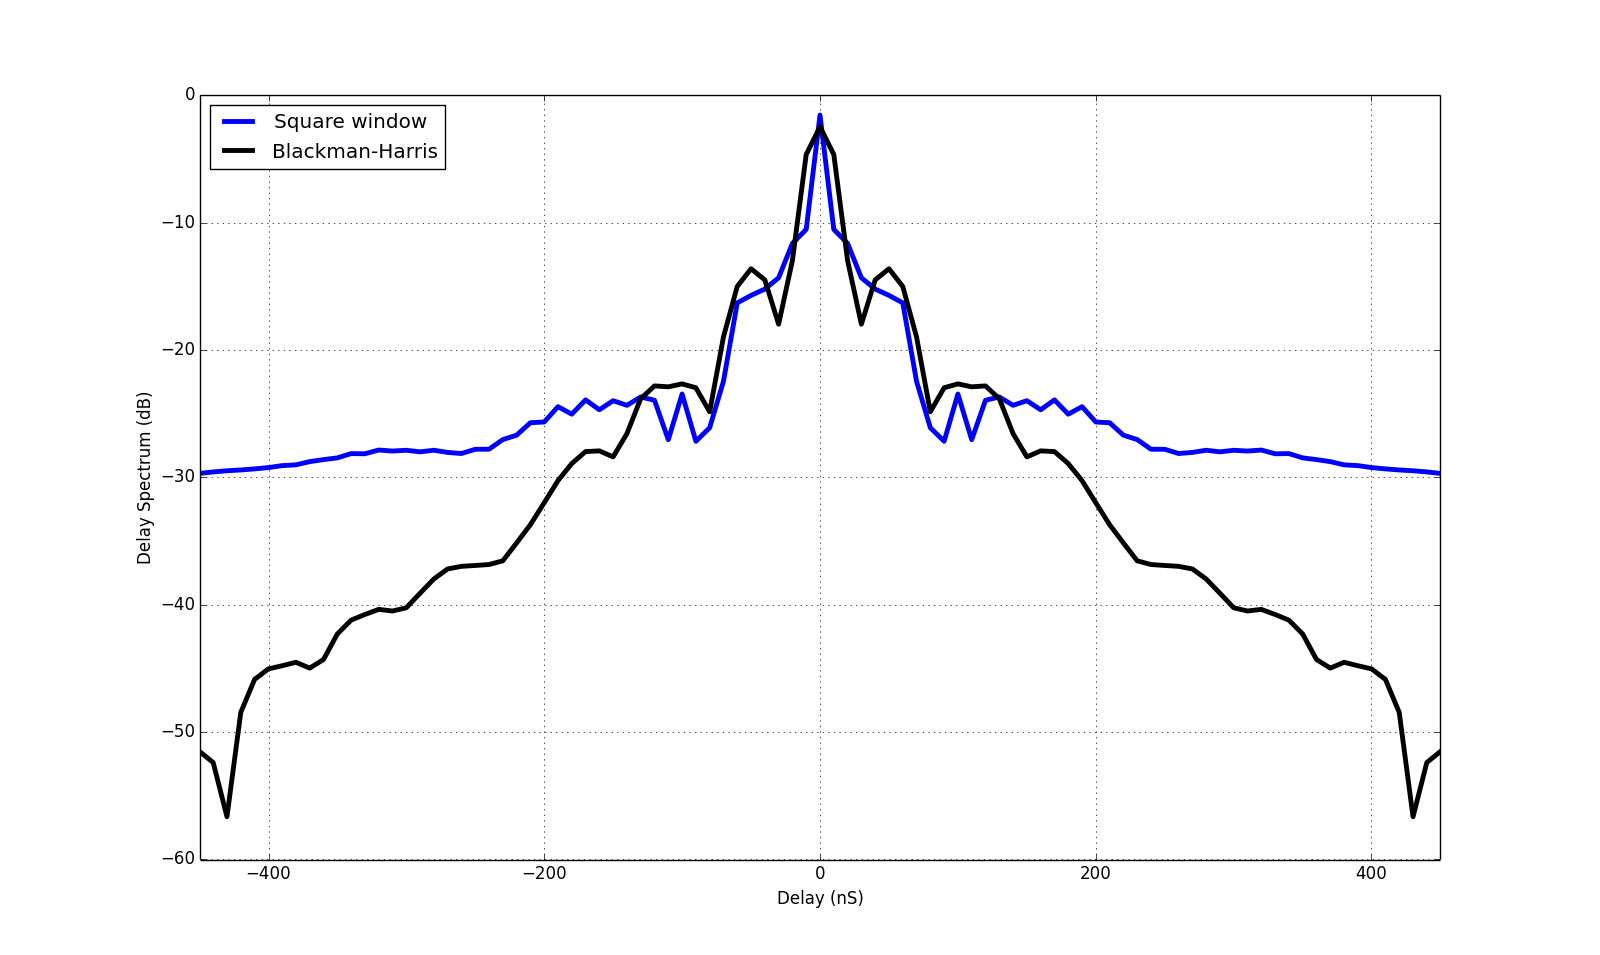
\includegraphics[width=\linewidth]{GB_reflectometry_part3/plot/ds_window.png}
\caption{Effect of finite bandwidth on estimation of delay spectrum: Blue line shows the delay spectrum of the HERA element computed from the measured data which is band limited between 100 to 200MHz. Green line shows the delay spectrum estimated from the same data set after multiplying the data by a Blackman Harris window. The delay spectrum of the windowed data set shows significant reduction in the instrument response at higher delays.}
\label{fig:window}
\end{figure} 

\subsection{\textbf{Multiple reflection between the feed and the backend.}}
Multiple reflections of the sky signal between the feed and the dish broadens the delay response of the instrument resulting in spill over of the smooth foreground power sky at higher delays. Another effect that have exact similar impact on the delay spectrum is the multiple reflection of the received signal between the feed output and the input of the analog backend and correlators. In our measurements, the feed output is connected to the VNA via a 50 feet long LMR 400 cable. This length correspond to a delay of $\approx 120~nS$ for the signals travelling through the cable. The delay spectrum of both feed and feed-dish assembly shows an enhanced feature at this delay indicating a reflection from the VNA input. We measure the VNA input reflections by disconnecting the feed and connecting an open load at the feed input of the cable. The measured return loss is shown in the figure \ref{fig:open_RL}. Since the electromagnetic wave travelling through a transmission line undergoes a $100\%$ reflections from an open ended transmission line, we compute the combined effect of the VNA input return loss along with the cable resistive loss from this measurement as shown in fiigure \ref{VNA_RL}. This results an important system design criterion for HERA. The VNA input return loss is found to be at a level of $-14$ to $-30dB$ across the measurement band. This is consistent with the matched provided by the commercially available RF connectors that are commonly used. This manifests itself in a peak in the delay spectrum which is $50~dB$ above the measurement noise floor. The delays at which this effect becomes dominant depends on the length of the cable. Due to finite return loss at the input of the backends, this effect will be present in all the observations and thus would impact the instrument delay spectrum. However, its effect could be reduced below the level where the foreground  achieving a return loss at the backend input is greater than at least $-30~dB$. 

\begin{figure*}[ht]
\begin{minipage}[b]{0.5\linewidth}
\centering
\includegraphics[angle=0, width=\linewidth]{plots/open_RL.png}
\end{minipage}
\hspace{0.1cm}
\begin{minipage}[b]{0.5\linewidth}
\centering
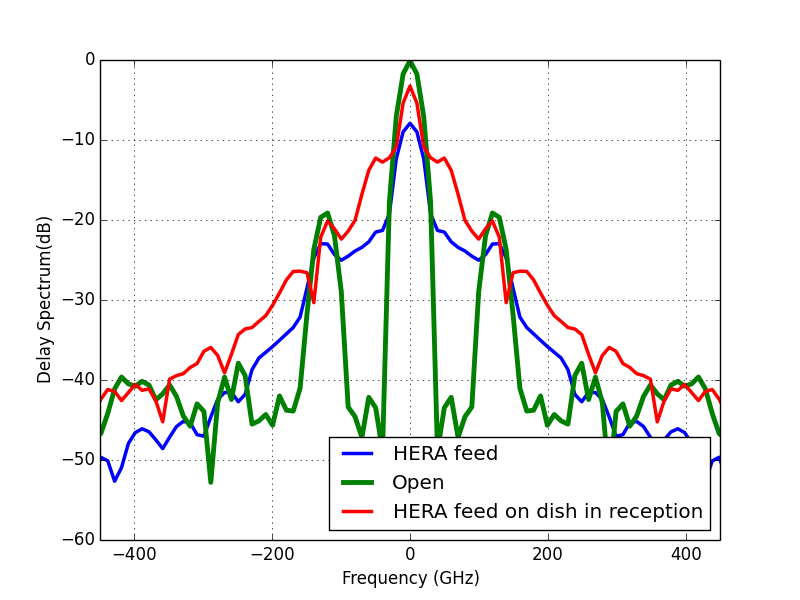
\includegraphics[angle=0, width=\linewidth]{plots/open_delay.png}
\end{minipage}
\caption{Left: Magnitude and phase of the return loss measured when the open load is connected at the feed input of the cable. Ideally, for an open load, the electromagnetic wave travelling through the transmission cable undergoes a $100\%$ reflections and magnitude of the return loss is $0dB$. However, due to the resistive loss in the cable, the a small part of the signal is dissipated in the cable resulting a smaller return loss.  Right: Delay spectrum of the open load that shows the multiple reflections at the VNA input. The delay spectrum of the feed and the feed-dish assembly is also plotted for comparison.}
\label{fig:open_RL}       
\end{figure*}

%While measuring the return loss of the dish-feed assembly, the signal transmitted by the VNA is reflected first off the feed. This is represented by $\Gamma_{f}$ in equation \ref{eq:power_ratio}. This essentially represents a mismatched impedance between the feed and the 50 Ohm transmission line. In the delay domain, this appears at the zero delay bin. This response is identical whether or not the feed is suspended on the dish. We can, therefore, quantify this response by measuring the feed return loss while the feed is kept on the ground facing the sky. This results in a feed return loss including the surrounding cage structure but excluding the dish response. While a fraction, $\Gamma_{f}$, of the power is reflected off the feed, $1+\Gamma_{f}$ gets transmitted. In the receiving mode, upon initial incidence, $\Gamma_{f}$ of the voltage is reflected back into free space while $1+\Gamma_{f}$ enters the feed, and, in the delay domain, this appears at the zero delay bin. Using the return loss measurement of the feed $(\Gamma_{f})$ and the return loss measurement, $s_{11}$, of the dish, the feed assembly is corrected via equation \ref{eq:power_ratio} for the zero delay component, and the quantity of interest ${I_{rec}\over I_{sky}}$ is estimated. 
%
%
%\begin{figure}[ht]
%\centering
%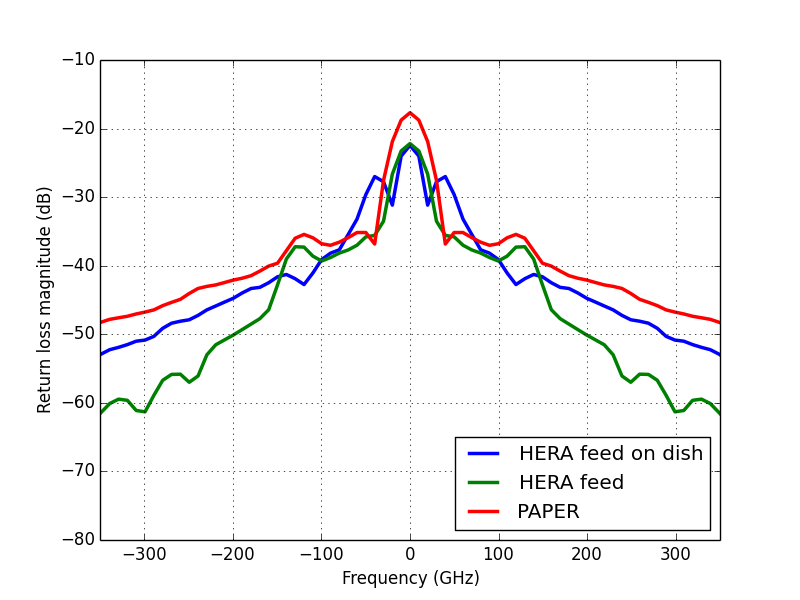
\includegraphics[width=\linewidth]{plots/delay_spectrum_100_200_BH.png}
%\caption{Delay spectrum of the HERA element, the PAPER element, and the HERA feed estimated by taking the Fourier transform of the measured return loss of power at the feed output. The HERA feed design is driven by the PAPER element with an improved response at all delays. The feed, when suspended on the dish, results in a more complex return loss, and the corresponding delay response is shown in the figure.} %Delay units are incorrect!!!! Should be ns not GHz!!!!
%\label{fig:delay_spectrum}
%\end{figure}

\section{\textbf{Effect of instrument delay spectrum on 21cm power spectrum measurements}}

21cm power spectrum measurements are limited by challenges posed by the low frequency radio foreground that is order of magnitude brighter than the expected power spectrum amplitude. While PAPER has established the till date the most stringent upper limit on the 21cm power spectrum measurement, the need for increased sensitivity called for increased collecting area per PAPER element. This has driven to the parabolic reflector antenna based design of the PAPER successor HERA where essentially the PAPER antenna with minor modification of the ground plane-side plane assembly works as the feed and thus having larger collecting area per element. Additional limitations on PAPER and its contemporaries are imposed by the spectral structure of the system response. Sky signal is frequency modulated by the system bandpass response. In delay spectrum technique of 21cm power spectrum estimation, sky signal is convolved with the system response in the delay domain. In this process of convolution, the frequency dependent system response with rapid frequency variation results in spreading of the smooth spectrum foreground of the sky signal to the delays in which EoR power spectrum is to be estimated. This essentially limits the capacity of any experiment to probe the smaller spatial scales of fluctuations. \\
	In a related series of papers, the spatial scales of fluctuation $(k_||)$ HERA element delay response has been studied via electromagnetic simulation (deBoer et al 2016) as well as via time domain simulation (Ewall-wice et al 2016). Figure \ref{fig:sim_em} and \ref{fig:sim_pk} shows the measurement presented this paper in comparison with the simulations. Simulations and measurements are in good agreement with each other upto around $60~ns$ up to which the structures in the delay domain are mostly caused due to signal reflections in the feed structure. Since the simulated return loss shows a better match of the antenna to the 50 Ohm transmission line. At zero delay , in case of simulation, almost $100\%$ of the sky signal is received whereas in case of measurements, this match is found to be less than $5~dB$ resulting in partial coupling of the sky signal to the system. Given all the reflections unaltered, if the matching in between the feed and the transmission line is improved by about $10~dB$, which is achievable in reality, the delay spectrum would improve substantially. This is plotted in grey. The work is currently under progress to improve the feed return loss at least by  $10dB$ (Eloy et al 2016 in prep?). Beyond $60~nS$ other multiple reflections manifests themselves at higher delays and the delay spectrum of the measurement and simulations begin to deviate from each other.\\
Thyagarajan et al 2016) has presented the detailed sensitivity calculations of HERA is using a comprehensive foreground model as well as model for EoR power spectrum for various simulated antenna element response. The sensitivity is quantified as a ratio of EoR signal power to the foreground power at various $\bold k_{\parallel}$ mode i.e at various delays. The theoretical limits for the level of foreground attenuation required relative to the EoR signal in order to reduce the foreground contaminations at the delay modes significant for power spectrum measurements are shown for three different lower limits of $k_\parallel$ values.  The response is computed for the redshift of $z=8.47$ at frequency $150~MHz$ over a bandwidth of $10~MHz$. This simulation shows the effect of chromatic antenna response and how that contaminates the delay modes beyond the horizon limit. Thus, this establishes a very stringent limits of required foreground attenuation relative to EoR signal which demands almost an ideal system performance. \\
%As shown in section (), multiple reflection in the antenna system generates multiple copies of the sky signal and thus results in additional foreground contaminations in the delay modes where EOR power spectrum is measurable in case of no reflections. Reflectometry measurements shows the relative strength with which the multiple copies of the signal shows up at various delays.

\begin{figure}
\centering
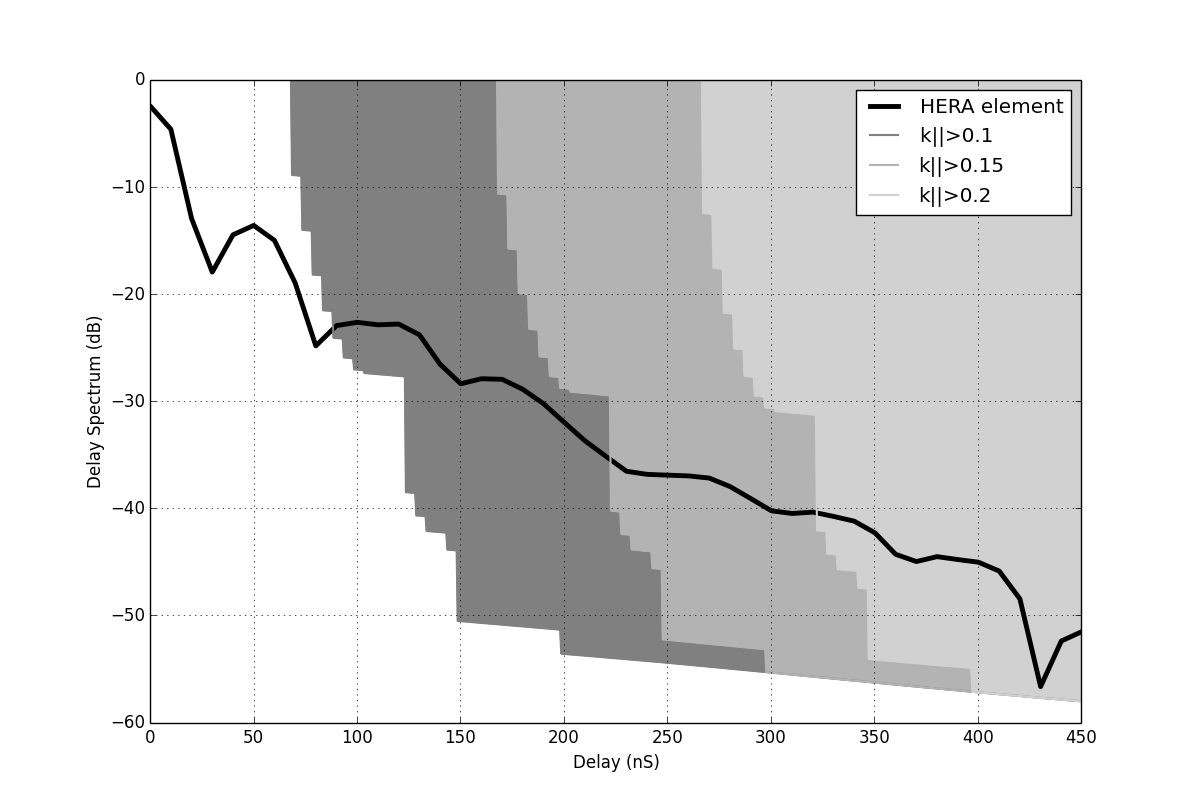
\includegraphics[width=\linewidth]{GB_reflectometry_part3/plot/HERA_ds_fg_sim.png}
\caption{Delay spectrum of HERA element estimated from the reflectometry measurements by a vector network analyser compared to the limits of foreground simulation (Thyagarajan et al).}
\label{fig:sim_fg_Nithya}
\end{figure}

The HERA analysis pipeline for power spectrum estimation exploits the inverse covariance weighting technique to reduce the foreground contribution to the measured visibility data. In the light of this analysis technique we further investigate the limits of required instrumental delay response from what is established by foreground simulation in Thyagarajan et al 2016. In the following section we briefly describe the power spectrum estimation technique used in HERA analysis and the inverse covariance weighting. In the next section we evaluate the estimated instrument delay response performance in the context of covariance weighting.

\subsection{Power spectrum estimation:}
HERA power spectrum estimation is done using the Optimal Quadratic Estimator (OQE) formalism that has been outlined in extensive detail in (Liu and Tegmark 2011), (Dillon et al 2013), (Liu et al 2014a,2014b), (Trott et al 2016), (Ali et al 2015). We briefly  describe the OQE formalism here.\\
HERA instrument aims at measuring the redshifted 21~cm power spectrum $P_{21}(k_\perp,k_\parallel)$, conventionally written as, 
\begin{equation}
\langle  \tilde T_{b}(\bold k) \tilde T_{b}^{*}(\bold k^{'}) \rangle = (2\pi)^{3} \delta (\bold k - \bold k^{'})P_{21}(k_\perp,k_\parallel)
\label{eq14}
\end{equation}

where $\langle  \tilde T_{b}(\bold k) \tilde T_{b}^{*}(\bold k^{'}) \rangle $ is the correlation function of the three dimensional spatial Fourier transform of the sky brightness temperature distribution $ \tilde T_{b}(\bold k)$, and $\delta$ is the Dirac delta function. While both $P_{21}(k_\perp,k_\parallel), \tilde T_{b}({\bold k})$ is continuous, the power spectrum could only be estimated at discrete values of $\bold k$. Observation frequency and bandwidth are so chosen that the power spectrum could e approximated as a constant and a piecewise continuous function of $\bold k$  which correspond to a thin shell in $\bold k$ space. This corresponds to the $k_{perp}$, $k_{parallel}$  values $a <k_{\perp} < a+1$, $b <k_{\parallel} < b+1$ where the indices a, b can assume M, N different values.  We denote the power spectrum as $\hat p_{\alpha}$ where alpha represents a particular $(M,N)$ value. Our analysis begins with a data vector $\bold x$. $\bold x$ is the list of visibilities measured at a given frequency over a certain bandwidth i.e for a given $k_{\parallel}$ mode for a given $\Delta \bold k $. The first estimate of power spectrum is written as, 

\begin{equation}
\hat q_{\alpha} = \bold x^{T} E^{\alpha} \bold x  - b^{\alpha}
\label{eq15}
\end{equation}

where $b_{\alpha}$ is a constant that assumes different values for each $\bold k$ and represents any additive noise power spectrum or residual foreground contamination to power spectrum estimate. $b_{\alpha}$ could be eliminated from the estimate by cross correlating two visibility data sets at two different times. $E^{\alpha}$ is a symmetric matrix operation denoting the Fourier transform of the data, binning, and foreground reduction. Various binning and foreground reduction technique would result in various different form of $E^{\alpha}$ resulting in estimates of $\hat p_{\alpha}$ with non identical statistics. A possible choice of $E^{\alpha}$ is
\begin{equation}
E^{\alpha} =  {1 \over 2} C^{-1} Q_{\alpha} C^{-1}
\label{eq16}
\end{equation} 

where $C = \langle \bold x \bold x^{t} \rangle$ is the covariance matrix of the data vector $\bold x$. $Q_{\alpha} \equiv {\delta C \over \delta p_{\alpha} } $ is a matrix operator that Fourier transforms the visibilities along the frequency axis and maps them into the $\bold k$ space for every M,N values. Finally, the normalized estimate of the power spectrum could be written as,  
\begin{equation}
\hat p_{\alpha} = M \hat q_{\alpha} 
\label{eq17}
\end{equation} 

Since $\hat p_{\alpha}$ is a discrete estimate of the true power spectrum $p_{\alpha}$, both are related by the window function matrix $W$, 
\begin{equation}
\hat p_{\alpha} = W p_{\alpha}
\label{eq18}
\end{equation} 

Hence, the estimated power spectrum $\hat p_{\alpha}$ for a given $k_{\perp}, k_{\parallel}$ values would have contribution for the nearby $k_{\perp}, k_{\parallel}$ values weighted by the window function. The wider the window function, the larger would be the contribution of the adjacent modes to the discrete power spectrum estimate. In general, therefore, $W$ is a non-diagonal matrix. Also, for a given choice of normalization matrix M, the window function W will be, 

\begin{equation}
 W = MF
 \label{eq19}
\end{equation} 

where , 
\begin{equation}
 F_{\alpha\beta} = \frac {1} { 2} [C^{-1}Q_{\alpha}C^{-1}Q_{\beta}]^{T}
 \label{eq20}
\end{equation} 
 is the Fisher matrix of the measured data. The choice of normalization matrix $M$ is critically important for the analysis. If $M = F^{-1}$, $W=I$ resulting in $\hat p_{\alpha} = p_{\alpha}$ i.e, estimated value of the power spectrum equals to the true power spectrum.\\
 The errors on the power spectrum estimate is given by the covariance of the band power which could be computed from the measured data as,  
\begin{eqnarray}
 C_{\alpha} & = & \langle \hat p_{\alpha} \hat p_{\alpha}^{T} \rangle - \langle \hat p_{\alpha} \rangle \langle \hat p_{\alpha}^{T} \rangle \nonumber\\
 		& = & MFM^{T}
\label{eq21}
 \end{eqnarray} 
 
 For a choice of $M = F^{-1}$, the covariance in the estimated band power is as large as $M$ resulting in highest error in estimation. Hence, the choice of the normalization matrix $M$ is critical in the analysis process since its precise form determines the vertical error bars in the estimate of power spectrum. 

\subsection{Inverse covariance weighting: revised delay spectrum limit}
The inverse variance weighting method is a method of aggregating two or more random variable to minimize the variance in their weighted average. In our case, the measured visibility is contributed by EoR, foreground and instrumental noise. Hence, the estimate of any of the constituent signal would benefit from if the measured data is weighted by the covariance of the individual components. This is reflected in our choice of the matrix $E^{\alpha}$.  $E^{\alpha} = {1 \over 2} C^{-1} Q_{\alpha} C^{-1}$ represents a weighting of the data vector $\bold x$ by inverse of its covariance. This results in the smallest vertical error bar in the power spectrum estimate $\hat p_{\alpha}$ (Reference Liu 2011). 
However, there no definite way to know the covariance of individual signal components prior to estimating them. In practice, the total covariance matrix $C$ is computed from the measured visibilities. It is a sum of covariances of the foreground, instrumental noise and the EoR signals. The highest covariance is rendered by the signal which is correlated over various frequency channels at all frequencies such as foreground. Hence, weighting the measured visibility by the inverse of the covariance results in order of magnitude reduction of foreground power against the EoR signal \\
 Combining the inverse covariance weighting formalism with the foreground simulation of Thyagarajan et al 2016, we derive a new limit on required foreground attenuation with respect to the EoR signal, required for power spectrum estimation using HERA measurements. The foreground model of Thyagarajan et al (2015a) is adopted wherein the diffused emission is accounted for using de Oliviera-Costa et al. 2008 and the point sources are modeled using NRAO VLA sky survey at 1.42 GHz(NVSS, Condon et al 1998) and Sydney University Molonglo Sky Survey (SUMSS; Bock et al 199;Mauch et al 2003.) at 843 MHz. The EoR signal model is derived from the 21cmFAST (Messinger et al 2011). The model parameters are kept same as what is used in Thyagarajan et al 2016 and Ewall-wice et all 2016. The EoR model parameters are listed below.\\
 Virial temperature of minimum mass of dark matter halos that host ionizing sources, $T_{vir}^{min} = 2*10^4 K$, Ionising efficiency $\eta = 20$, Mean Free Path of UV photons $R_{mfp} = 15Mpc.$ For these model parameter values, the redshift of $50\%$ reionization is predicted to be at $z = 8.5$ at 150MHz.\\
We use the reflectometry measurements, corrected for the antenna response in the receiving mode, to compute the visibilities (eq 13) for the given model of the foreground, the EoR and the system noise. These visibilities formed the complex data vector $\bold x$. We compute the covariance matrix $C$ from the simulated data. $\bold x$ is then multiplied by the inverse of the covariance matrix. This step essentially weighs down the foreground contribution to the measured data. Once Fourier transformed, the delay spectrum of the simulated data is constituted by linear super position of the delay spectrum of the foreground, the EoR signal.  We again compute the EoR to foreground power ratio which is now smaller than what is estimated in Thyagarajan et al 2016 as shown in fig:\ref{fig:sim_fg_revised}. 
\begin{figure*}[ht]
\centering
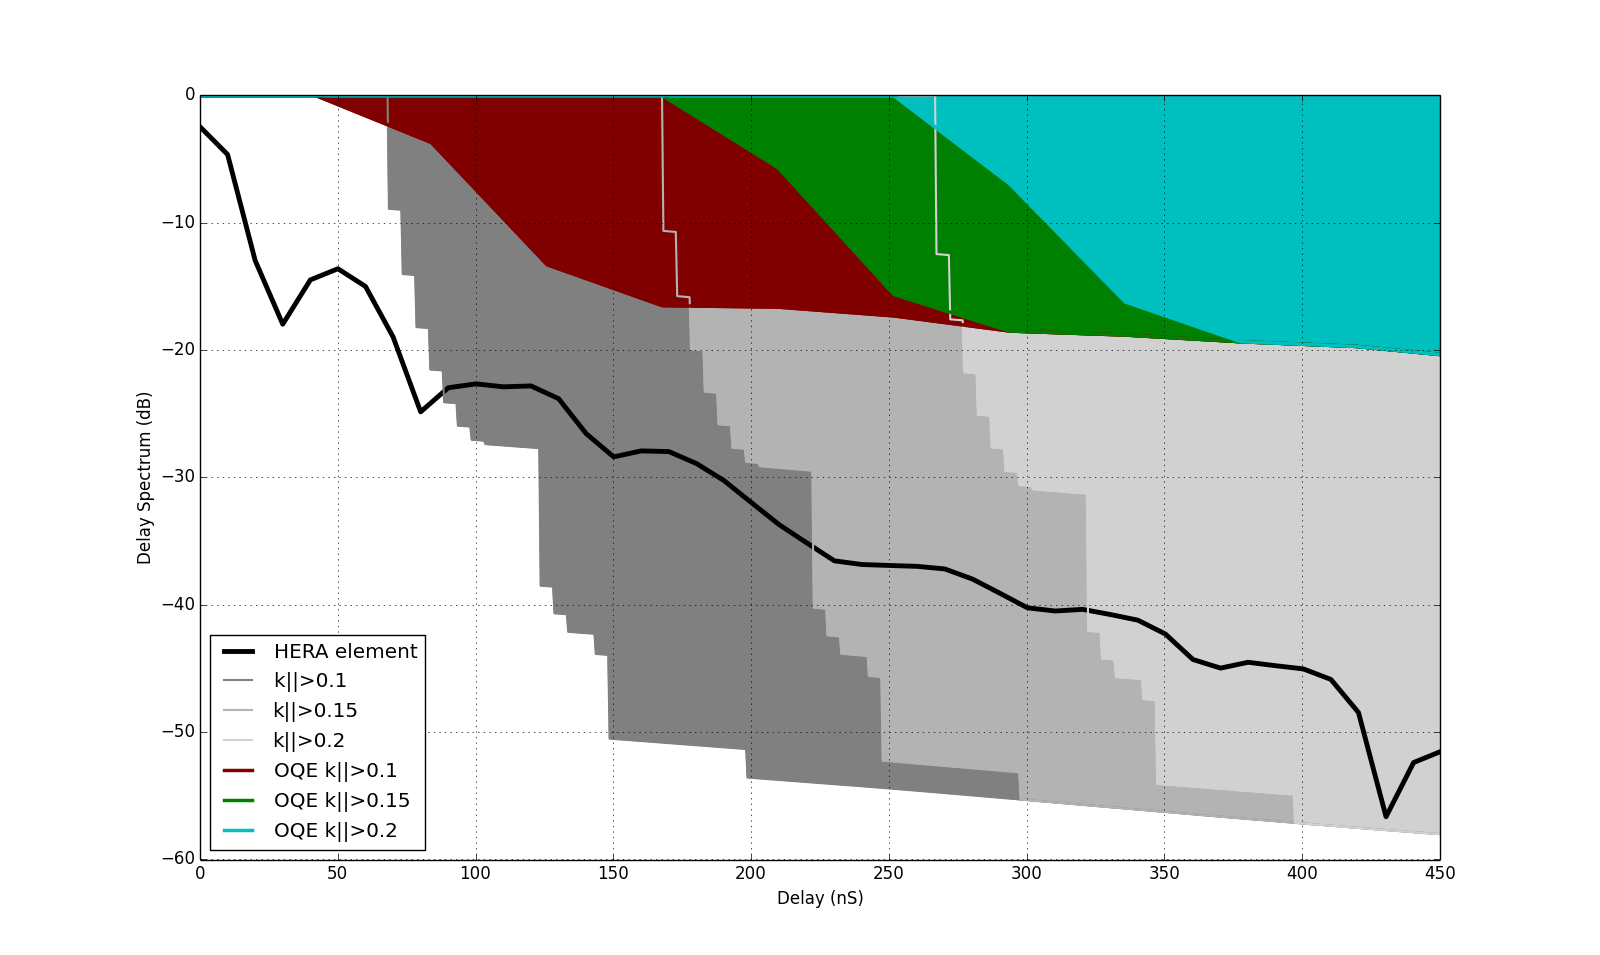
\includegraphics[width=\linewidth]{GB_reflectometry_part3/plot/HERA_ds_fg_sim_rev.png}
\caption{Delay spectrum of HERA element estimated from the reflectometry measurements by a vector network analyzer. The colored region shows the revised EoR to foreground power ratio in comparison to the measurements and the foreground simulation presented in (Thyagarajan et al 2016).}
\label{fig:sim_fg_revised}
\end{figure*}
This demonstrates that the performance of the HERA element performance, in conjunction with the inverse covariance method of foreground suppression, qualifies the system for its the science goal it is designed for, irrespective of its chromatic response generated due to multiple reflections in the system.


%Covariance matrix $C$ is computed from the simulated visibility data. Next, the data vector $\bold $ that consists of the complex simulated visibilities, is weighted by the computed covariance of the data. 
%instrument delay response for power spectrum measurements. With inverse covariance weighting a %foreground suppression of about 30dB could be achieved that results in room for substantial %performance degradation and yet a successful measurement of 21~cm power spectrum. Our %measurements, evaluated in the light of these limits shows that the HERA is not limited by either its %systematics. With only delay spectrum technique, it is capable of detecting the EoR power spectrum %for the $k_{\parallel}$ modes as low as $k_{\parallel}>=0.2$. If combined with the inverse covariance %weighting formalism of foreground suppression, the instrument performs well below the limits of %foreground suppression. We briefly describe the inverse covariance weighting formalism below.
%\subsection{Inverse covariance weighting}
%The 21 cm delay spectrum estimate and thus the 21~cm power spectrum, consists of three main components, the foreground power spectrum $\hat p_{FG}$, the EoR power spectrum $\hat p_{EoR}$and the noise power spectrum of the instrument.
%\begin{equation}
%\hat p =  \hat p_{FG} + \hat p_{EoR}+ \hat p_{noise}
%\end{equation}
%In the inverse-variance weighting, two or more random variables are aggregated to minimize the variance of the weighted average. Hence, weighting the estimated delay spectrum with the inverse variance of the foreground reduces the foreground contaminations in the measurements. 
%would  for power spectrum measurements, especially at smaller spatial scales of fluctuation i.e lower values of $k_{\parallel}$.




\section{\textbf{Conclusion}}
The interplay between the extremely bright sky signal with the system response has remained somewhat undermined for the first generation 21cm experiments such as MWA, LOFAR, PAPER. With the theory of redshifted 21cm experiments have very well evolved, it is absolute necessity now to quantify the instrumental limits of these measurement in order to produce a believable power spectrum estimates.
In this paper, we studied the performance of a HERA element in both frequency as well as delay domain. The effects of multiple reflections  in a HERA feed-dish assembly is investigated in detail and their effects on the measured visibility as well as delay spectrum is estimated.  The delay-domain performance of the HERA dish is central to HERA's function as a power spectrum instrument. Reflectometry measurements characterised HERA's performance in this domain, and as Equation \ref{eq10} shows, these measurements must be adjusted for a difference in transmission/reflection
at the first feed encounter in order to be interpreted as the delay response of a feed relative to an incident
plane wave from the sky.  It is also shown that the choice of windowing function is critical for accurately measuring the
antenna delay response at higher delays, where sidelobes from much higher amplitude responses at small delays can easily
dominate.  Blackman-Harris window is found to be generally adequate while square windowing functions are not.
Given the critical nature of the windowing function, it is recommended that all reflectometry measurements be performed in the
frequency domain, so that the data could be Fourier transformed with the appropriate window.
The delay spectrum estimates are then compared with the electromagnetic as well as time domain simulation of the HERA element~\citep{Ewall-Wice_et_al2016}, ~\citep{ddboer_et_al2016}. The same is then compared with the foreground simulation of~\cite{Thyagarajan_et_al2015}. The performance is also evaluated in the light of HERA power spectrum estimation technique using inverse covariance weighting formalism. 
Taken all together, we summarise that the HERA antenna element, with a PAPER-style crossed dipole feed and cylindrical cage the instrument delay spectrum very well satisfies the criteria necessary to meet its science goal. 

%\bibliography{biblio}{}
\bibliographystyle{apj}
\bibliography{Reference}{}

\end{document}

